\documentclass[12pt]{book}
\usepackage[left=1in,right=1in,top=1in,bottom=1in]{geometry}
\usepackage{latexsym}
\usepackage{listings}
\lstset{breaklines=true, language=Python, showspaces=false, showstringspaces=false}
\usepackage{wrapfig,subfig,graphicx}
\usepackage{textcomp}

\begin{document}

%\author{Maritza Mallek}
\title{Modeling Historical Range of Variability and Future Land Management Scenarios in the Yuba River Watershed, Tahoe National Forest}
\date{December 2014}

\section*{Outline}
\subsection{Spatial Data Preparation}
Xeric/Mesic Gradient preparation\\
YHR Type Selection\\
Eveg Layer Selection\\
Scale and Extent\\
Scripts and tools used for spatial data prep\\
some of this will be redundant with the rmlands spatial data pdf\\
Age

\subsection{landcover type descriptions and models}
Primary sources for text (e.g. landfire, whr, feis, Cal veg book)\\
Primary sources for model values (e.g. landfire, expert opinion)\\
generation of succession probabilities\\

\subsection{general notes}
may be worth it to include general description of how and when we involved FS folks\\
District vs. Ecology Group vs. Hugh vs. other advisors\\

\subsection{original goal list}

The original set of work to be done was:
\begin{enumerate}
\item{Create state transition models for each Yuba River cover type. Hopefully they can be based largely on the LandFire cover types.}
\item{Analyze existing cover types and LandFire cover types}
\item{Evaluate the quality of the data: for example, conduct a compositional analysis in GIS and determine the relative similarity between the EVeg, PNV, and Wieslander vegetation layers.}
\item{Do a lit review to collate data on the pertinent disturbance regimes.}
\end{enumerate}

%\frontmatter 
%\tableofcontents 
\include{preface} 

\mainmatter 
%\include{1_InputLayerPrep} 
\chapter{Methods}
\section{Study Area}
\label{sec:studyarea}

\begin{figure}
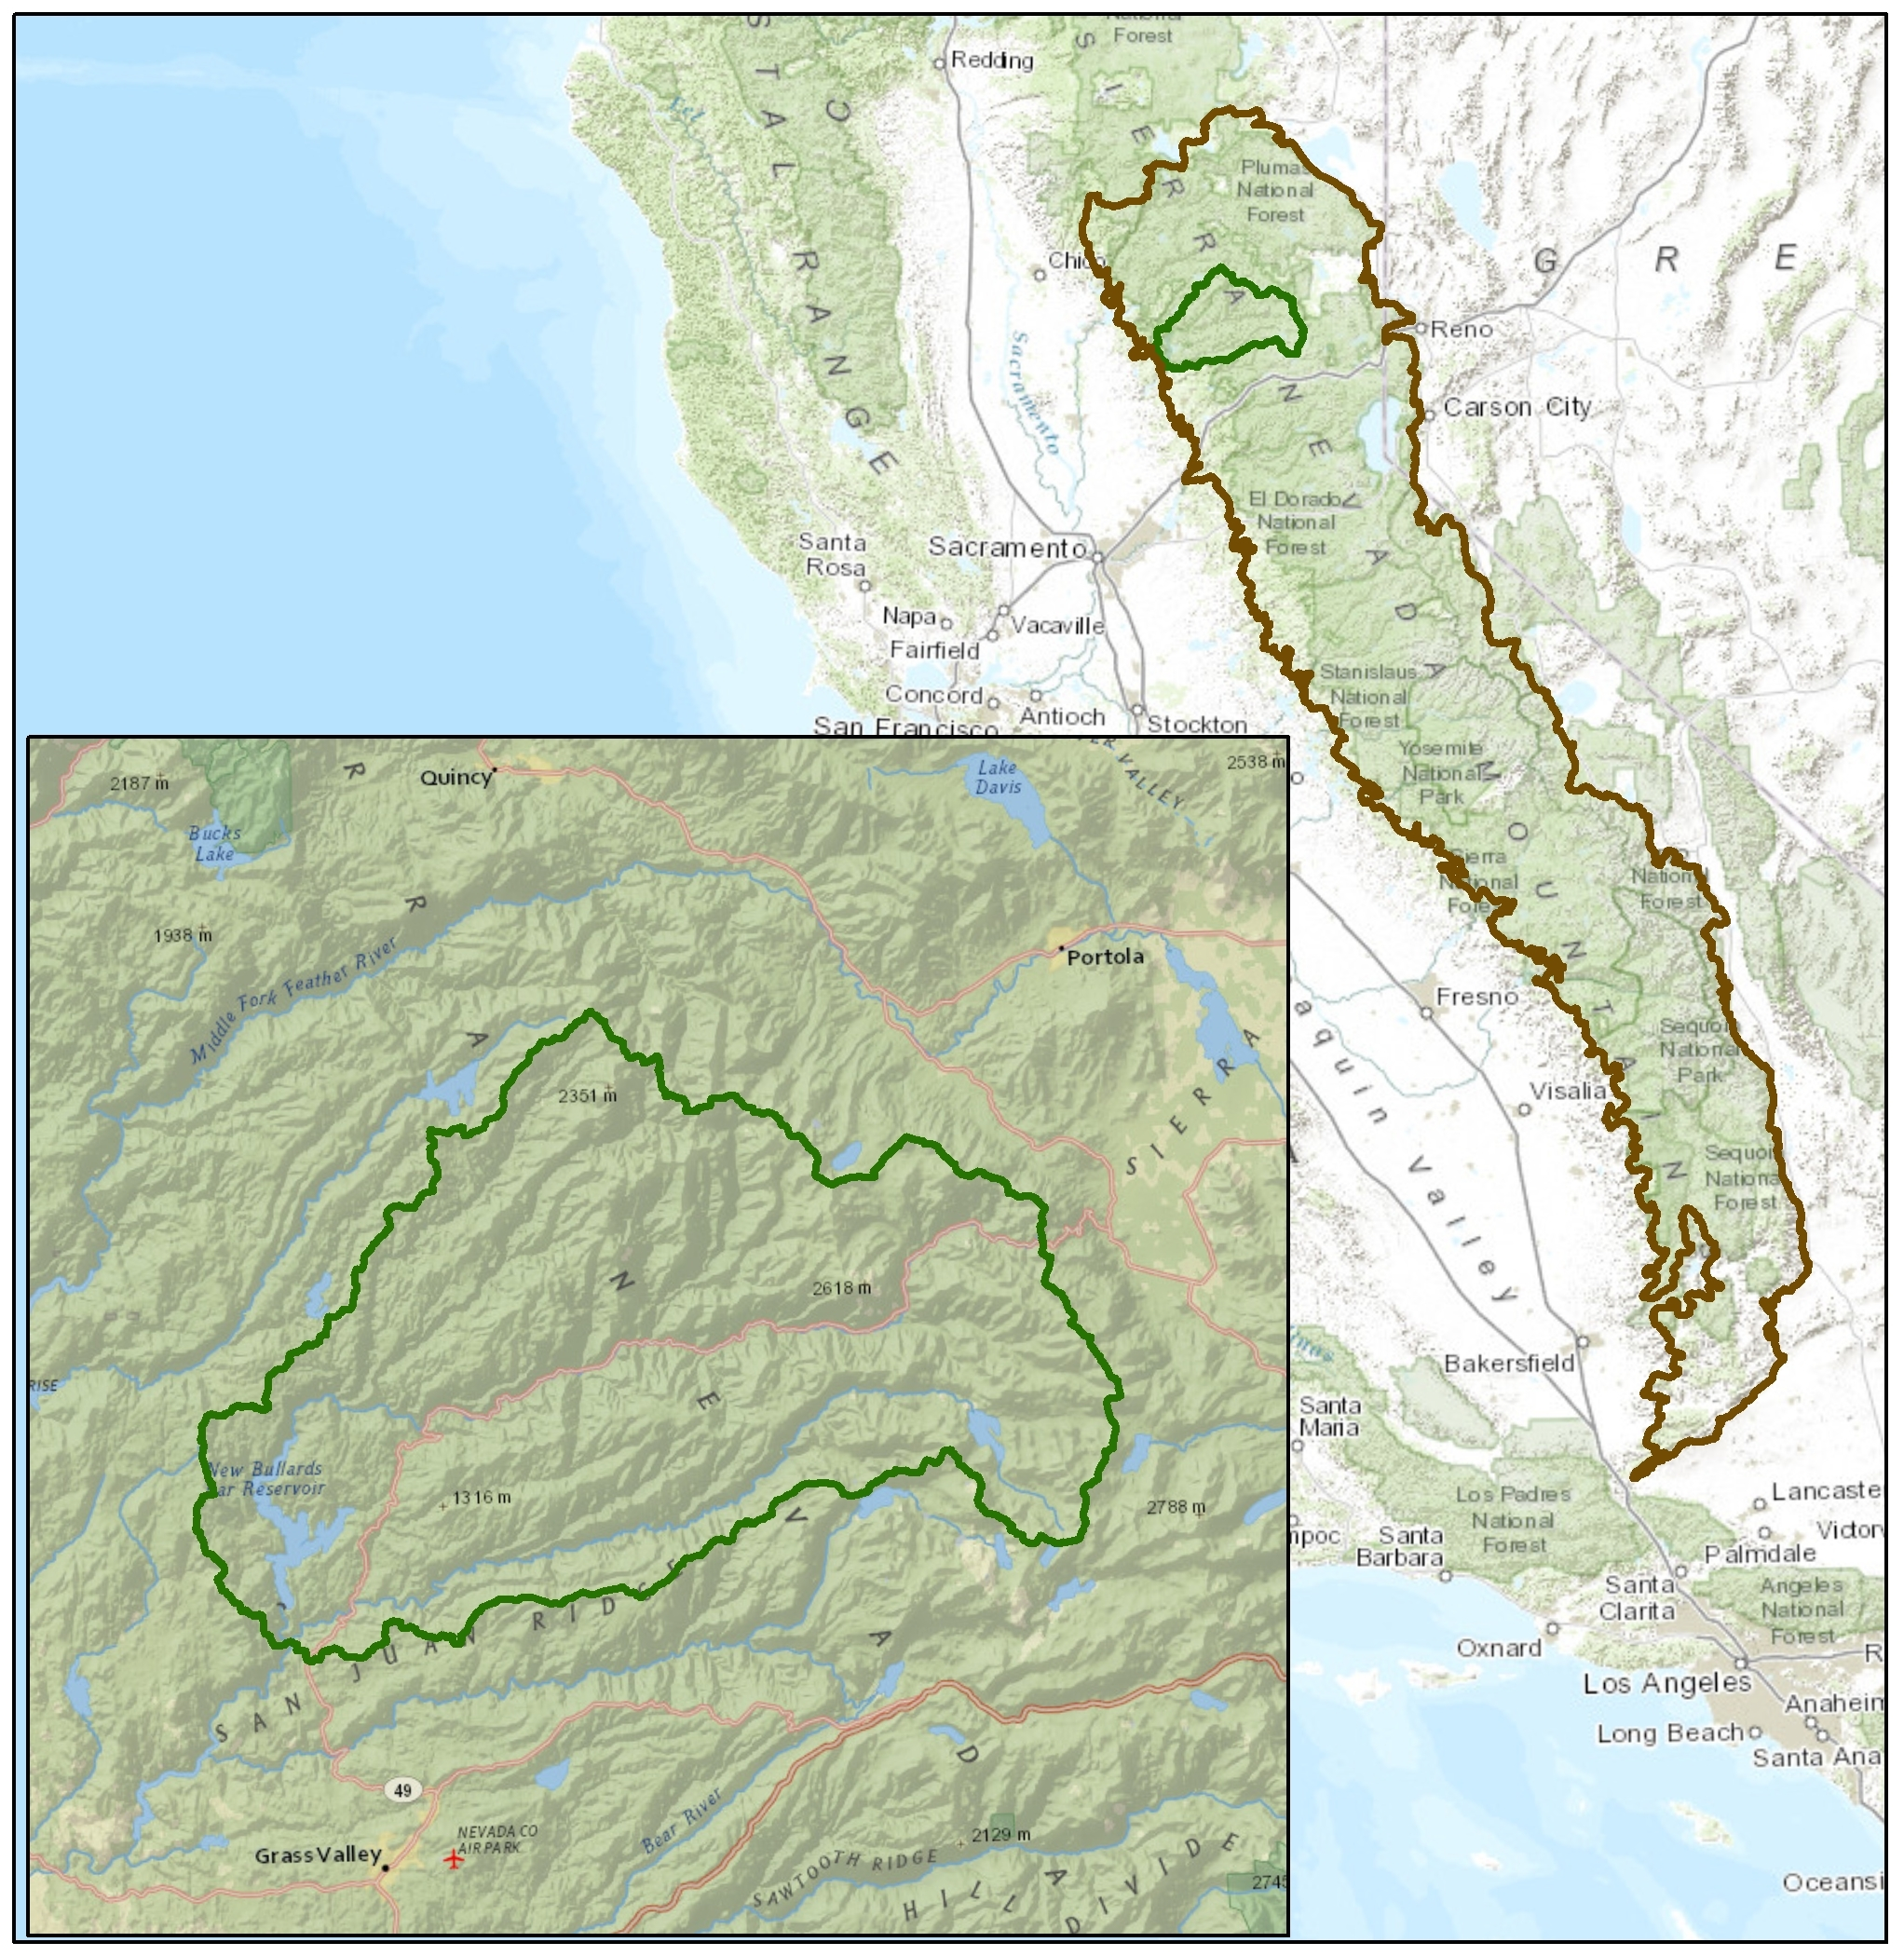
\includegraphics[width=\textwidth]{images/ecoregionprojectarea.jpg}
\caption{The Sierra Nevada Ecoregion is outlined in brown. The project landscape (outlined in green) is located in the northern extent of the Sierra Nevada on the Tahoe National Forest, comprising the Yuba River watershed.}
\label{projectarea}
\end{figure}

The Sierra Nevada is a major North American mountain range, located east of California's Central Valley and extending from Fredonyer Pass in the north to southern Kern County in the south. Much of the Sierra Nevada is reserved as federally-held public land, managed by the U.S. Forest Service, Bureau of Land Management, and the National Park Service. The Plumas and Tahoe National Forests are located in the northern portion of the Sierra Nevada. The project landscape (see Figure~\ref{projectarea}) is located on the northern part of the Tahoe National Forest, on the Yuba River and Sierraville Ranger Districts, and comprises about 181,550 hectares. It is composed of a set of three HUC-5 watersheds, the Upper North Yuba River, the Middle Yuba River, and the Lower North Yuba River, collectively referred to in this document as the Upper Yuba River watershed. 

The topography of the project landscape consists of rugged mountains incised by two major and a few minor river drainages. Elevation ranges from about 350 to 2500 meters. The area receives 30--260 cm of precipitation annually, most of which falls as snow in the middle to upper elevations (Storer and Usinger 1963). Some areas in the mid-elevation band receive high precipitation compared to the region, resulting in patches of exceptionally productive forest (Alan Doerr, pers. comm.). Vegetation is tremendously diverse and changes slowly along an elevational gradient and in response to local changes in drainage, aspect, and soil structure. Grasslands, chaparral, oak woodlands, mixed conifer forests, and subalpine forests are all found within the study area. Many species exhibit fire-adapted traits, such as resprouting from roots after a fire (e.g. tanoak), fire-induced germination (e.g. manzanita), or thick bark (e.g. ponderosa pine). 

Prior to European settlement, wildfire was a major source of disturbance on the landscape, shaping the composition and configuration of vegetation in the Forest. Fires were primarily lightning-caused, although indigenous peoples are thought to have set fires for vegetation management, especially in the lower elevations. In general, fire was frequent, with a mean rotation as short as 20 years in Ponderosa Pine-dominated forests. Wetter mixed conifer areas are predicted to have had a mean fire rotation of 30 years. Fire rotation is thought to increase gradually with elevation. For example, mesic Red Fir forests, which exist around 2,000 feet higher in elevation than Ponderosa Pine forests, had a mean fire rotation of 60 years. Variance around these means can be significant, as some parts of the forest experience fire much more frequently, while other escape fire for long periods. In general, regardless of vegetation type, high mortality fires were thought to be rare, with the vast majority of fires killing under 70\% of overstory trees. Under this disturbance regime, stand-replacing fire initiated early development conditions on the landscape. Low mortality fire tended to open forest canopies, especially in more xeric parts of the forest, while vegetation succession closed them again. The rarity of high mortality fire allowed large forest stands to succeed into late development and old growth conditions. \todo{How to cite this? At the end of the paragraph or repeatedly in it?}

The arrival of Europeans in the 1850s sparked a transformation of this landscape as people harvested timber, extracted gold using hydraulic mining techniques, and suppressed wildfires (Storer and Usinger 1963). Forestry, mining, grazing, and dozens of recreational activities, including hunting, mountain biking, and hiking continue to take place on the Tahoe National Forest. Fifteen allotments exist within the project area for both cattle and sheep grazing. In addition, 231,368 hectares inside of the project area have non-Forest Service ownership. Many of these lands were privately held, often by timber companies, before the Forest was created. In addition, many public lands were given to the Central Pacific Railroad in the late 19th century, and this ``checkerboard'' ownership pattern persists today (Figure~\ref{ownership}). Mining of gold and other minerals also continues. These activities affect and interact with ongoing vegetation succession and disturbance processes in the area. \todo{info easily found on forest website - need to cite?}

\begin{figure}[!htbp]
\centering
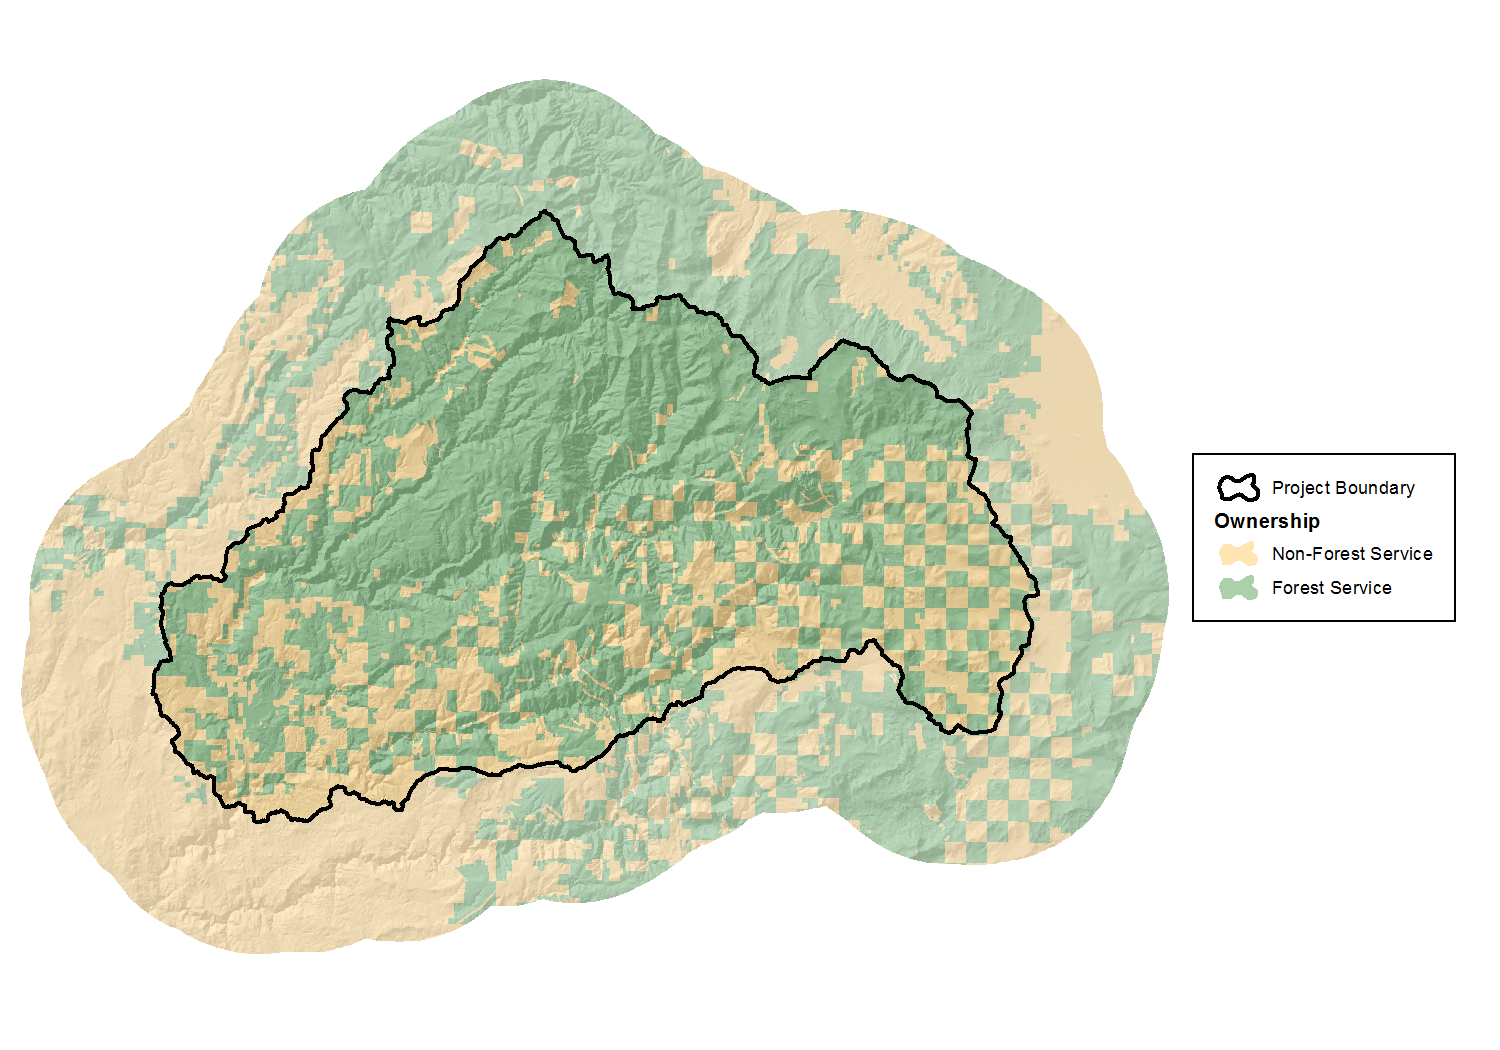
\includegraphics[width=0.8\textwidth]{/Users/mmallek/Tahoe/Report2/images/ownership.png}
\caption{Map distinguishing between National Forest lands and lands held by other entities (including private, industry, and other public land).} 
\label{ownership}
\end{figure}

The Tahoe National Forest has an active fire management program, and maintains a cooperative agreement with the State of California to help fight wildfires on the non-Forest Service lands located with the Forest boundary. In the recent history of the forest, very few acres have burned, with the exception of 1960, when approximately 100,000 acres burned on the Forest. The low burned acreage corresponds with fairly high fire starts (both human- and lightning-caused) [Forest Plan]. Fire suppression has lead to an increase in the amount of dead and downed fuels in the forest (SNFramework).

Logging has been a major human impact on the Forest since European settlement. Clearcutting, shelterwood, salvage cutting, and plantation management have been major components of timber management on the TNF for several decades. More recently, group cut strategies replaced clearcutting as a management alternative. Together with fire suppression, timber management on the Forest has effected changes in forest composition. In general, shade intolerant species such as ponderosa pine, sugar pine, and Douglas fir have become less common, while shade tolerant species, especially white fir, have become more predominant [1990 Forest Plan]. In the last 20 years, timber sales in the Sierra Nevada have dropped drastically, but on the Tahoe National Forests timber sale levels have fluctuated both up and down (although annual sawtimber sold has decreased similarly to other Sierran Forests).


\section{Modeling Framework}
\label{sec:modelframe}

\section{Historic Range of Variability}

\subsection{Input Layers}
\label{subsec:hrvinputlayers}

\paragraph{Data Structure} \textsc{RMLands} uses raster GeoTiffs (.tif files) as its data structure. Rasters are based on uniform square units called cells (or pixels). Each cell represents an actual portion of geographic space, where each cell has a defined X and Y value that corresponds to the coordinates defined by the projection. For example, in the Universal Transverse Mercator (UTM) projection, the grid that covers the entire Tahoe and Plumas National Forests project area is in UTM Zone 10 North and covers an area defined by a range of X and Y values (minimum and maximum).\footnote{Latitude and longitude are commonly pictured when describing coordinates. In such cases the X value refers to longitude and Y refers to latitude. However, because we use UTMs in this project, the correct convention is actually that the X value is the Easting and the Y value is the Northing. For simplicity we discuss X and Y only in this document.} In the Yuba River watershed landscape, each grid cell is 30 meters on a side (i.e., 900 m$^2$ or 0.09 ha), and the input grid measures 2910 by 2245 pixels. All grids must be single-attribute, signed integer grids. In other words, each cell is assigned a single class value, where valid class values are positive or negative whole numbers. All grids are created in ArcMap and saved as GeoTitff files before being input to the model. 

\paragraph{Raster layer alignment} \textsc{RMLands} requires that all grids are perfectly aligned. This means that not only must all grids have the same cell size and the same numbers of rows and columns, but the cells need to occupy the exact same geographic space and have the same number of total cells. \textsc{RMLands} requires that all input grids are perfectly aligned. We accomplished this by setting the Extent and Snap Raster to the same parameters whenever we manipulated the layers in ArcMap. This ``base'' spatial layer was created by taking the primary elevation layer used on the Tahoe National Forest, resampling it to a 30 meter grid, and clipping its extent to match that of the buffered project area.

The input layers are: cover, condition, age, aspect, slope, elevation, streams, roads, and condition-age.

\todo{Could also put all the maps of these layers on one page, as part of 1 large figure. Either 4 or 6 to a page.}

\subsubsection{Cover} The \emph{cover} layer represents land cover type, which is often but not always the vegetation type (i.e. cover types include not only Lodgepole Pine, but also Barren, and Agriculture). \emph{Cover} does not change over time, and is used to define several model parameters, including susceptibility to disturbance initiation or spread, and potential transitions between \emph{condition} classes undergone by cells within a particular cover type.

Cover represents land cover type. Typically, cover type is based on the potential or current natural vegetation of a site and may include both natural and anthropogenic cover types. For example, cover types include not only Lodgepole Pine, Sierran Mixed Conifer, and Red Fir, but also Barren and Agriculture. Cover affects virtually every process in \textsc{RMLands}. Succession pathways are defined uniquely for each cover type, susceptibility to natural disturbances varies among cover types, and suitability or eligibility for various vegetation treatments varies among cover types. Cover is a \emph{static} grid. Specifically, cover provides a fixed template upon which disturbance and succession processes play out over time. The cover type of a cell does not change over time; it is constant. All cells within the project boundary must be assigned a cover type; i.e., there can be no missing data or ``background'' within the project boundary. NODATA is reserved for all cells outside the project boundary.

The source for the cover layer is the Region 5 Existing Vegetation Layer (``EVeg''), mapped to the CALVEG classification developed by the Region's Ecology Program in 1978. The CALVEG types in the project area are specific to the North Sierra mapping Zone. Within the project area, the EVeg layer was developed based on three separate efforts: a satellite-based imagery analysis in 2000, and two orthoimagery analysis completed by contracting firms in 2005. Generally, specific cover type names were derived from the California Fire Return Interval Departure (FRID) report by Safford et al. \todo{Citation}

\paragraph{Alternative Cover Layers}
The original intent of our team was to utilize two separate cover layers: one for the historical reference period, and one for the current period to be used in projections of future scenarios. Two layers were identified as potentially suitable for the historic analysis: a map created from forest survey and inventory efforts under Albert Wieslander conducted between 1928 and 1940 (``Wieslander'') \todo{cite CEC}, and a map of Potential Natural Vegetation created by a Forest Service Enterprise Team for the Tahoe National Forest in the 2000s (``PNV''). Our intent was to use the PNV, Wieslander, or a combination thereof to derive the land cover layer for the HRV phase of the project. 

In order to validate the historical maps, we needed to develop a crosswalk between the vegetation type methodologies for the EVeg, PNV, and Wieslander maps. We also examined the spatial consistency in cover types across the maps. With significant assistance from the Tahoe National Forest, we attempted to create a crosswalk from these maps to the set of land cover types to be used in the project. However, we were unable to develop a consistent and comprehensive set of rules for this purpose. A major reason for this is that both the PNV and Wieslander maps used species lists, rather than assemblages (like in CalVeg and LandFire). For example, Sierran mixed conifer forests do not appear as a dominant ``cover type'' in the PNV map. The Wieslander maps do contain an internal crosswalk to a mixed conifer alliance, but only rarely. 

In addition, the PNV map contained a more significant error: we learned that, for the purposes of the modeling used to create the PNV map, ``potential natural vegetation'' meant the so-called ``climax'' community that would develop in the complete absence of disturbance, regardless of whether that disturbance was human-caused or natural. Since we are seeking to mimic the natural historic range of variability, we decided to discard this layer. The Wieslander map had its own issues. Most problematic was the non-systematic spatial error of up to 300 meters, which meant it would not be suitable for comparing specific locations. In addition, crosswalking precisely was impossible because coded vegetation was not necessarily in order of most prevalent vegetation, but instead prioritized tree species of shrubs, and commercially important trees over others. As an example from the handbook states, a plot consisting of 75\% \emph{Quercus kelloggi} (black oak), 15\% \emph{Pinus ponderosa} (ponderosa pine), and 10\% \emph{Pinus lambertiana} (grey pine) would be coded as ponderosa pine, grey pine, black oak. Consequently, the Wieslander map is also not a reliable predictor of land cover type without extensive review of the original data and maps, which would be beyond the scope of this project. 

To confirm these problmes, we examined the overlap in land cover types between different maps in ArcGIS. In general, the overlap between EVeg and either the PNV or the Wieslander layers was no better than random, and in many cases it was worse. We decided, in conjunction with Tahoe National Forest staff, to proceed using only the EVeg map, and omit the calibration period of the model from our analysis of the characteristics of the HRV. This ensured that our analysis of future management scenarios and comparison of spatial metrics between those results and the HRV results was credible.
% in retrospect I wonder if we should have analyzed the configuration more. in the end the biggest problem was probably the lack of crosswalk, since a precise spatial equivalence wasn't assumed.

\paragraph{Selection of Specific Cover Types}
In the early stages of this project, the team created a suite of land cover types based roughly on the Wildlife Habitat Relationships (WHR) types used in California and by Forest Service managers and planners. These consisted of the WHR types with a few additional types where additional specificity or refinement was desired. For example, Red Fir was split up into two subtypes. The original concept was to begin with the WHR types and modify them as needed based on other attributes in the EVeg layer. However, creating a crosswalk from WHR to the project-specific types also proved problematic. First, we realized that the WHR values were actually derived from the CalVeg species alliances included in the EVeg layer, but the methodlogy used was unavailable or missing. The crosswalks we did find \todo{cite} were not mutually exclusive and all-inclusive, and do not always make ecological sense. This is probably due in part to the fact that WHR is not a mapping classification. It is always derived secondarily. So, we were unable to create consistent rules for mapping from WHR to other types. Others have encountered similar issues:

\begin{quote}
WHR has been less successful in differentiating between vegetation types. Because the habitat types are inconsistently defined, a broad familiarity with its detailed descriptions is needed to differentiate among types of similar structure. Although mappers have constructed rules for discriminating among types, difficulties still remain because species dominance varies substantially within some types and broad overlaps in dominant plants occur among types. Other problems arise due to the small number of classes and the inconsistencies in scale among them \todo{(T. Veg of Cal)}
\end{quote}

With Tahoe National Forest staff we decided to instead base our land cover types on, at the first order, Presettlement Fire Regime (PFR) types as defined in the Fire Return Interval Departure (FRID)report by Safford et al. \todo{cite}. The PFR types, as part of the FRID, were developed through the scientific process and underwent peer review. We used the methodology from the FRID rather than using the second-order WHR classification and trying to reverse-engineer it to fit into our custom land cover types. Thus we created a new structure of cover types in a nested regime, moving from PFR (the coarsest aggregation of CalVeg types, which included a direct crosswalk from them to PFR types), to Biophysical Settings from LandFire (which were also crosswalked to PFR types in the FRID report), and finally to various local types not otherwise represented, such as xeric and mesic variants of cover types like Montane Hardwood, and aspen variants, such as Red Fir - Aspen. A mutually exclusive and all-inclusive crosswalk for each land cover type used in this analysis to a single LandFire Biophysical Setting and Presettlement Fire Regime type thus exists.

Extensive geoprocessing was required to prepare the EVeg layer for use in \textsc{RMLands}. Beyond converting the vector data to a raster format, further analysis was required to distinguish east- and west-side areas from one another, and generate the cover type modifications that the team agreed on. Aspen types were created by overlaying an aspen layer onto the vegetation layer and creating combined types (``type-aspen'')where appropriate. Areas mapped as a vegetation type characteristic of early seral (e.g. chaparral) were analyzed and assigned an appropriate forested cover type. Ultramafic types were created by overlaying a geology layer onto the vegetation layer and performing a similar processing step to create ``type-ultramafic''. Finally, for the Sierran Mixed Conifer and Red Fir cover types, which cover broad swaths of land across elevation and aspect, a xeric to mesic gradient was developed in conjunction with local experts and applied, creating ``type-mesic'' and ``type-xeric''. 

Ultimately, 31 cover types were generated for the buffered project area, as listed in Table~\ref{covertable} and shown in Figure~\ref{covermap}. A thorough description of geoprocessing steps necessary to recreate this data layer is available \todo{in forthcoming document?}. As Table~\ref{covertable} shows, most cover types occupy a small extent of the project area. The cover types with an extent of less than 1000 ha within the core project area may have statistically unreliable results; this problem increases as the extent of given cover type decreases. We caution against attempting to make inferences for these less common cover types. However, because the nine cover types that do occur over at least 1000 ha represent approximately 93\% of the core project area, we have high confidence in the landscape-level results.

%%%%%%%%%%%%%%%%%%%%%%
%%% COVER TABLE %%%%%%
%%%%%%%%%%%%%%%%%%%%%%
\small
\begin{table}[!htbp]
\caption{List of land cover types developed for this project. Included are the cover type abbreviation, full cover type name, and total area in the buffered project landscape in both acres and hectares.}
\label{covertable}
\begin{tabular}{@{}lllll@{}}
\toprule
\textbf{\begin{tabular}[c]{@{}l@{}}Land \\ Cover \\ Value\end{tabular}} & \textbf{\begin{tabular}[c]{@{}l@{}}Land Cover \\ Abbreviation\end{tabular}} & \textbf{Land Cover Name}                              & \textbf{\begin{tabular}[c]{@{}l@{}}Area \\ Core Only\\ (Hectares)\end{tabular}} & \textbf{\begin{tabular}[c]{@{}l@{}}Area\\ Core+Buffer\\ (Hectares)\end{tabular}} \\ \midrule
\rowcolor[HTML]{CAD6BA} 
1                                                           & AGR                                                                & Agriculture                                  & 16                                                          & 5,416                                                      \\
2                                                           & BAR                                                                & Barren                                       & 2665                                                        & 8,751                                                      \\
\rowcolor[HTML]{CAD6BA} 
3                                                           & CMM                                                                & Curl-leaf Mountain Mahogany                  & 18                                                          & 41                                                         \\
4                                                           & GRASS                                                              & Grassland                                    & 1379                                                        & 4,617                                                      \\
\rowcolor[HTML]{CAD6BA} 
5                                                           & LPN                                                                & Lodgepole Pine                               & 837                                                         & 2,816                                                      \\
6                                                           & LPN\_ASP                                                           & Lodgepole Pine with Aspen                    & 8                                                           & 31                                                         \\
\rowcolor[HTML]{CAD6BA} 
7                                                           & LSG                                                                & Black and Low Sagebrush                      & 0                                                           & 5                                                          \\
8                                                           & MED                                                                & Meadow                                       & 1201                                                        & 3,435                                                      \\
\rowcolor[HTML]{CAD6BA} 
9                                                           & MEG\_M                                                             & Mixed Evergreen - Mesic                      & 7273                                                        & 13,547                                                     \\
10                                                          & MEG\_U                                                             & Mixed Evergreen - Ultramafic                 & 604                                                         & 1,655                                                      \\
\rowcolor[HTML]{CAD6BA} 
11                                                          & MEG\_X                                                             & Mixed Evergreen - Xeric                      & 6768                                                        & 13,771                                                     \\
12                                                          & MRIP                                                               & Montane Riparian                             & 732                                                         & 2,216                                                      \\
\rowcolor[HTML]{CAD6BA} 
13                                                          & OAK                                                                & Oak Woodland                                 & 19                                                          & 4,186                                                      \\
14                                                          & OCFW                                                               & Oak-Conifer Forest and Woodland              & 23729                                                       & 56,941                                                     \\
\rowcolor[HTML]{CAD6BA} 
15                                                          & OCFW\_U                                                            & \begin{tabular}[c]{@{}l@{}}Oak-Conifer Forest and \\ Woodland -  Ultramafic\end{tabular} & 1060                                                   & 2,185                                                      \\
16                                                          & RFR\_ASP                                                           & Red Fir with Aspen                           & 0     		                                              & 34                                                         \\
\rowcolor[HTML]{CAD6BA} 
17                                                          & RFR\_M                                                             & Red Fir - Mesic                              & 8563  		                                              & 19,626                                                     \\
18                                                          & RFR\_U                                                             & Red Fir - Ultramafic                         & 294   		                                              & 321                                                        \\
\rowcolor[HTML]{CAD6BA} 
19                                                          & RFR\_X                                                             & Red Fir - Xeric                              & 7493  		                                              & 9,989                                                      \\
20                                                          & SAGE                                                               & Big Safebrush                                & 0     		                                              & 1,600                                                      \\
\rowcolor[HTML]{CAD6BA} 
21                                                          & SCN                                                                & Subalpine Conifer                            & 638   		                                              & 12,543                                                     \\
22                                                          & SCN\_ASP                                                           & Subalpine Conifer with Aspen                 & 0     		                                              & 6                                                          \\
\rowcolor[HTML]{CAD6BA} 
23                                                          & SMC\_ASP                                                           & Sierran Mixed Conifer with Aspen             & 58    		                                              & 121                                                        \\
24                                                          & SMC\_M                                                             & Sierran Mixed Conifer - Mesic                & 57853 		                                              & 133,920                                                    \\
\rowcolor[HTML]{CAD6BA} 
25                                                          & SMC\_U                                                             & Sierran Mixed Conifer - Ultramafic           & 4124  		                                              & 9,774                                                      \\
26                                                          & SMC\_X                                                             & Sierran Mixed Conifer - Xeric                & 52198 		                                              & 91,443                                                     \\
\rowcolor[HTML]{CAD6BA} 
27                                                          & URB                                                                & Urban                                        & 114   		                                              & 782                                                        \\
28                                                          & WAT                                                                & Water                                        & 4058  		                                              & 8,212                                                      \\
\rowcolor[HTML]{CAD6BA} 
29                                                          & WWP                                                                & Western White Pine                           & 273   		                                              & 510                                                        \\
30                                                          & YPN                                                                & Yellow Pine                                  & 0     		                                              & 10,499                                                     \\
\rowcolor[HTML]{CAD6BA} 
31                                                          & YPN\_ASP                                                           & Yellow Pine with Aspen                       & 0     		                                              & 3                                                          \\ \bottomrule
\end{tabular}
\end{table}
\normalsize

%\begin{verbatim}
%YHR	CellCount	Landcover3
%1	60173		AGR
%2	97233		BAR
%3	454			CMM
%4	51302		GRASS
%5	31289		LPN
%6	349			LPN_ASP
%7	50			LSG
%8	38171		MED
%9	150520		MEG_M
%10	18388		MEG_U
%11	153011		MEG_X
%12	24627		MRIP
%13	46514		OAK
%14	632677		OCFW
%15	24275		OCFW_U
%16	381			RFR_ASP
%17	218070		RFR_M
%18	3564		RFR_U
%19	110989		RFR_X
%20	17773		SAGE
%21	139365		SCN
%22	69			SCN_ASP
%23	1341		SMC_ASP
%24	1488003		SMC_M
%25	108605		SMC_U
%26	1016037		SMC_X
%27	8693		URB
%28	91245		WAT
%29	5668		WWP
%30 116653		YPN
%31	34			YPN_ASP
%\end{verbatim}

\begin{figure}[!htbp]
\centering
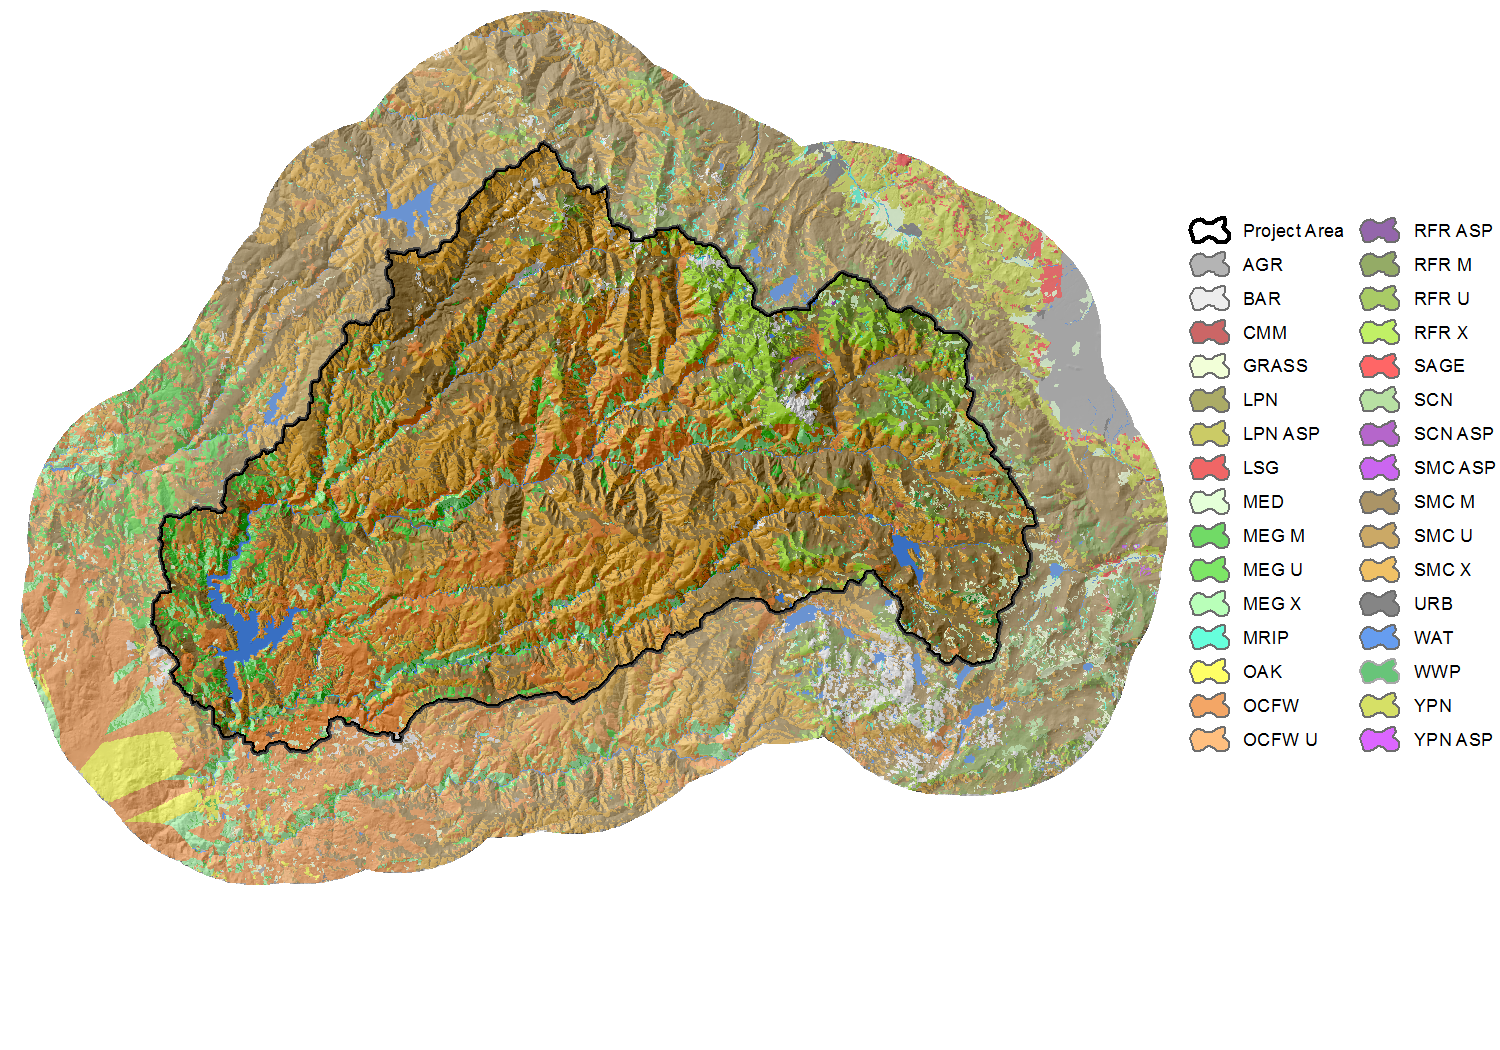
\includegraphics[height=0.4\textheight]{/Users/mmallek/Tahoe/Report2/images/cover.png}
\caption{Cover Type Map for the project area. Also shows the 10 km buffer from the project area boundary. See Table~\ref{covertable} for full land cover type names.} 
\label{covermap}
\end{figure}


\subsubsection{Condition}
Condition (or stand condition) class represents the structural condition of vegetation for cover types that undergo succession. Condition is a representation of discrete seral stages of stand development as identified by experts, which may vary considerably among cover types. It affects virtually every process in \textsc{RMLands}. In particular, transitions among condition classes during stand development define the succession pathways for each cover type. In addition, condition can be specified as a factor affecting susceptibility to natural disturbances and suitability (or eligibility) for vegetation treatments. Condition is a \emph{dynamic} grid; cell values change over time during the simulation in response to disturbance and succession processes. Ultimately, the combination of condition and cover defines the categorical classification of the landscape that provides the framework for characterizing vegetation patterns and dynamics. All cells within the project boundary are assigned a condition class; i.e., there is no missing data or ``background'' within the project boundary. However, some cover types (e.g., Urban, Agriculture, Meadow, etc.) may not have multiple condition classes and can be assigned a common value.

The source for the condition layer is the Region 5 Existing Vegetation Layer, mapped to the CALVEG classification developed by the Region's Ecology Program in 1978. Within the project area, the Existing Vegetation Layer was developed based on three separate efforts: a satellite-based imagery analysis in 2000, and two orthoimagery analysis completed by contracting firms in 2005. All members of the team discussed potential attributes to be used for this classification, and identified attributes for tree diameter at breast height (DBH) and cover from above (CFA) to classify pixels into early, middle, or late development, and open, moderate, and closed canopy. In this application, aspen and shrub types have condition classes that differ from that of the remaining forest types. The other forested types use a consistent set of condition classes.

Extensive geoprocessing was required to prepare this layer for \textsc{RMLands}. Beyond converting the vector data to a raster format, further analysis was required to update the layer to a year 2010 condition. Spatial data on wildfire and timber management history was used to provide a more accurate assessment of condition based on estimated stand age. In addition, areas currently mapped as chaparral in the Existing Vegetation Layer were assigned to the early development stage. The full set of condition classes is provided in Table~\ref{condtable} and depicted in Figure~\ref{conditionmap}.

%%%%%%%%%%%%%%%%%%%%%%
%%% CONDITION TABLE %%
%%%%%%%%%%%%%%%%%%%%%%

\begin{table}[!htbp]
\centering
\caption{List of condition classes developed for this project. Condition classes describe developmental stage (e.g. ``early'') and canopy closure (e.g. ``open''). Included are the condition class codes, abbreviations, and full names.}
\label{condtable}
\begin{tabular}{@{}lll@{}}
\toprule
\textbf{\begin{tabular}[c]{@{}l@{}}Condition Class \\ Value\end{tabular}} & \textbf{\begin{tabular}[c]{@{}l@{}}Condition Class \\ Abbreviation\end{tabular}} & \textbf{\begin{tabular}[c]{@{}l@{}}Condition Class  \\ Name\end{tabular}} \\ \midrule
\rowcolor[HTML]{CAD6BA} 
0                              & NS                                    & Non-Seral                     				 \\
10                             & EARLY\_ALL                            & Early Development - All                   	 \\
\rowcolor[HTML]{CAD6BA} 
20                             & MID\_CL                               & Mid Development - Closed                    \\
21                             & MID\_MOD                              & Mid Development - Moderate                  \\
\rowcolor[HTML]{CAD6BA} 
22                             & MID\_OP                               & Mid Development - Open                      \\
30                             & LATE\_CL                              & Late Development - Closed                   \\
\rowcolor[HTML]{CAD6BA} 
31                             & LATE\_MOD                             & Late Development - Moderate                 \\
32                             & LATE\_CL                              & Late Development - Open                     \\
\rowcolor[HTML]{CAD6BA} 
40                             & EARLY\_ASP                            & Early Development - Aspen                   \\
41                             & MID\_ASP                              & Mid Development - Aspen                     \\
\rowcolor[HTML]{CAD6BA} 
42                             & MID\_AC                               & Mid Development - Aspen Conifer             \\
43                             & LATE\_CA                              & Late Development - Conifer Aspen            \\ \bottomrule
\end{tabular}
\end{table}

\begin{figure}[!htbp]
\centering
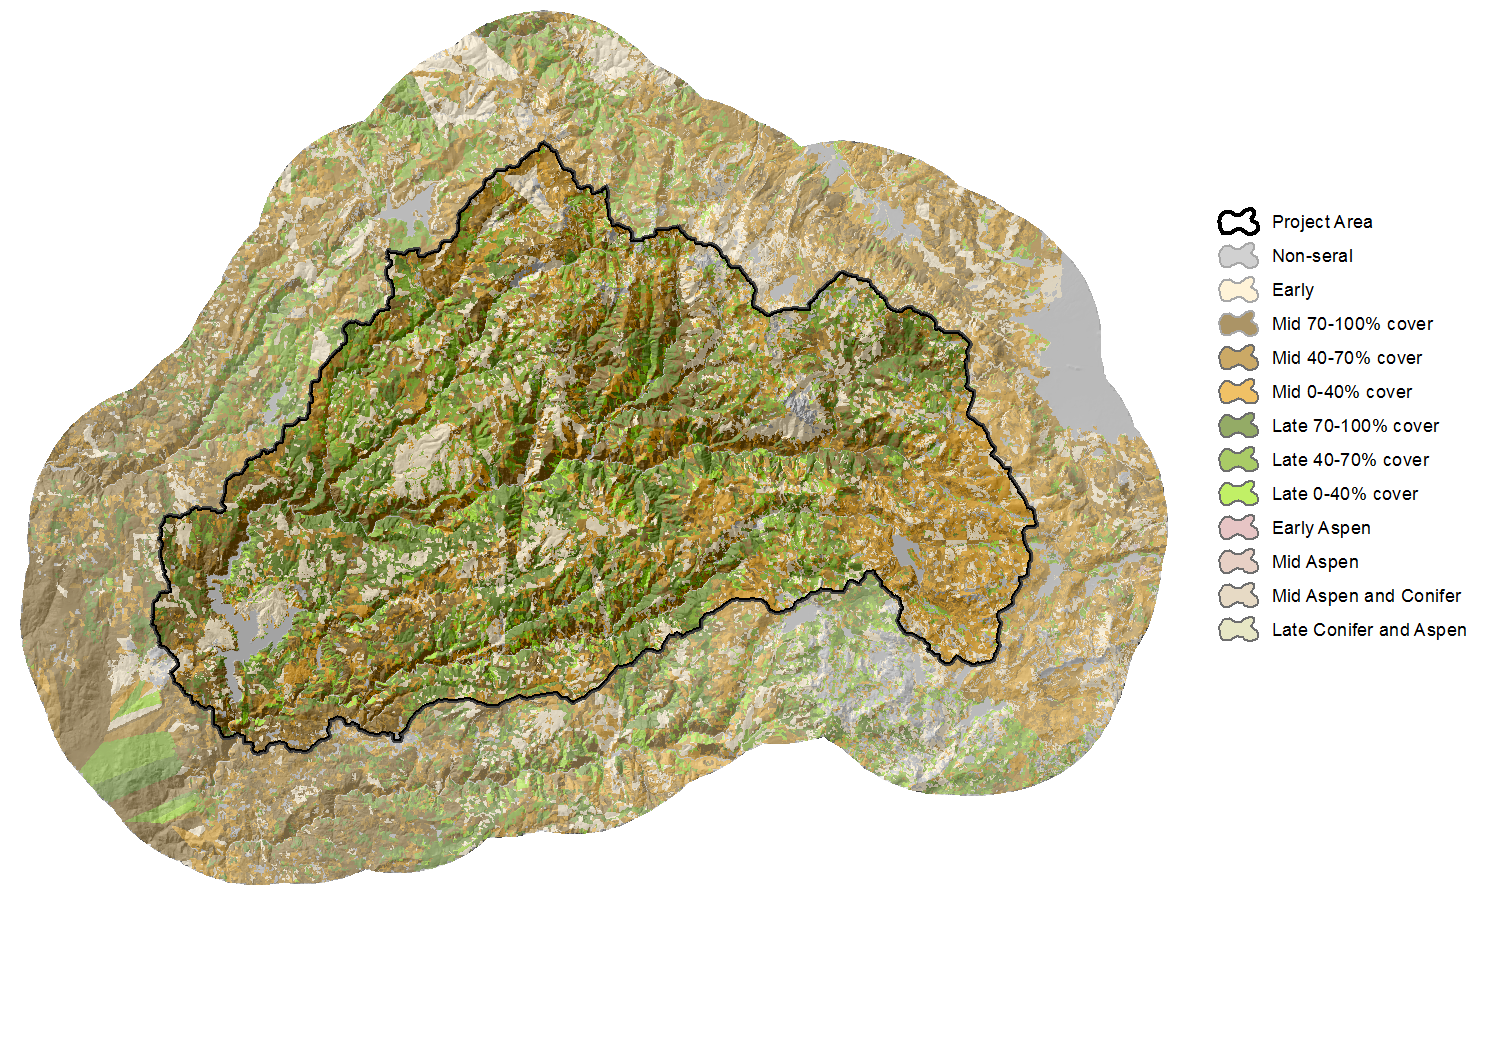
\includegraphics[height=0.4\textheight]{/Users/mmallek/Tahoe/Report2/images/condition.png}
\caption{Condition Class Map for the project area. Also shows the 10 km buffer from the project area boundary.} 
\label{conditionmap}
\end{figure}

\subsubsection{Age}
Age represents the number of years since stand origin (i.e., the number of years since the last stand-replacing disturbance), which is not necessarily the age of the oldest plant individuals in the stand. In some circumstances the age since stand origin can greatly exceed the age of the oldest individual plants (e.g., old-growth stands). It affects a variety of processes in \textsc{RMLands}, including succession transitions and susceptibility to disturbance. Age is a \emph{dynamic} grid; cell values change over time during the simulation in response to disturbance and succession processes. Age values can be any positive whole number, although any precision less than the length of the model time step (5 years) is inconsequential. In this application, we rounded all modeled and derived ages to the nearest five years. A ``no age'' value (99998) is assigned to all non-vegetated and non-seral cover types.

While Age is potentially an important variable in \textsc{RMLands}---for example, it is a factor influencing succession transitions and can provide a basis for summarizing the range of variability in vegetation conditions---the \emph{initial} age condition is a transient state that gets modified quickly during the simulation in response to disturbance and successsion processes. Therefore, the initial age structure of the landscape may be of little importance in a long-term simulation, as long as we properly account for the model equilibration period (i.e., the period it takes the age structure of the landscape to stabilize given the disturbance regime).

In this application, we used data from stand exams dating to the 1960s and from recent Forest Service Region 5 Ecology group survey plots to estimate stand age across the buffered project area. We then interpolated that information across the landscape. Due to insufficient data, we were unable to disaggregate the data below the landscape scale to cover type or another more finely resolved classification. We also acknowledge that the stand exam and modern veg plots do not constitute a true sample and were conducted almost exclusively in mid-mature and mature stands of commercially viable trees, thus skewing the results to some unquantifiable degree.

We updated the interpolated data with wildfire and timber management history, and assigned ages to types coded as chaparral in the Existing Vegetation layer to the midpoint of the age spread of early development for the forest cover type to which it was converted. Remaining ages out of compliance with allowed ages for the corresponding condition of a given cell were modified to be in compliance, based on the assumption that the condition class assignment was more accurate that the interpolated age information. The input Age layer, showing the map at timestep 0, is shown in Figure~\ref{agemap}.

\begin{figure}[htbp]
\centering
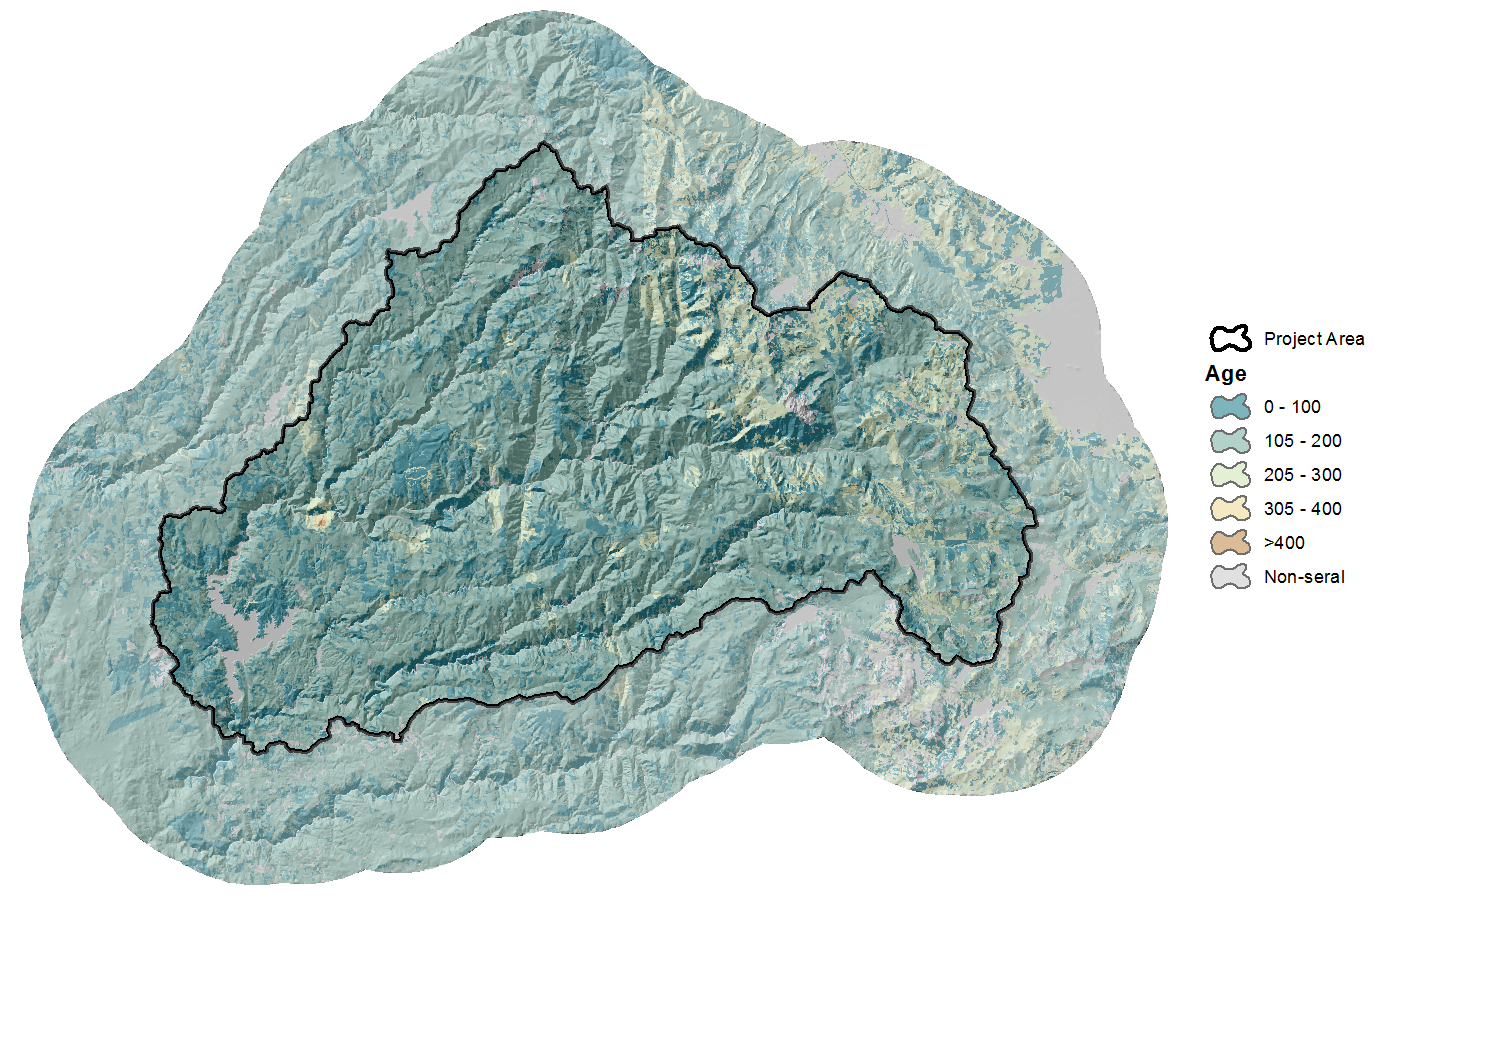
\includegraphics[height=0.4\textheight]{/Users/mmallek/Tahoe/Report2/images/age.png}
\caption{Age map at Timestep 0 for the project area. Also shows the 10 km buffer from the project area boundary.} 
\label{agemap}
\end{figure}

\subsubsection{Condition-Age}
Condition-Age represents the age since transitioning to the current condition. In \textsc{RMLands} it affects most transitions between condition classes: typically there is a threshold condition age below which transitions do not occur. After creating both the condition and age layers, we used a Python function to derive condition-age based on the youngest possible age for a cell of that cover and condition. For example, if we determine that a particular cell on the landscape has a cover type of Lodgepole Pine, condition of Mid Development Closed, and age of 50 years, we take the minimum age for that cover-condition combination (10 years old), and subtract it from the age to arrive at a condition-age of 40. The final, original map for the initial condition-age is shown in Figure~\ref{condagemap}.

\begin{figure}[htbp]
\centering
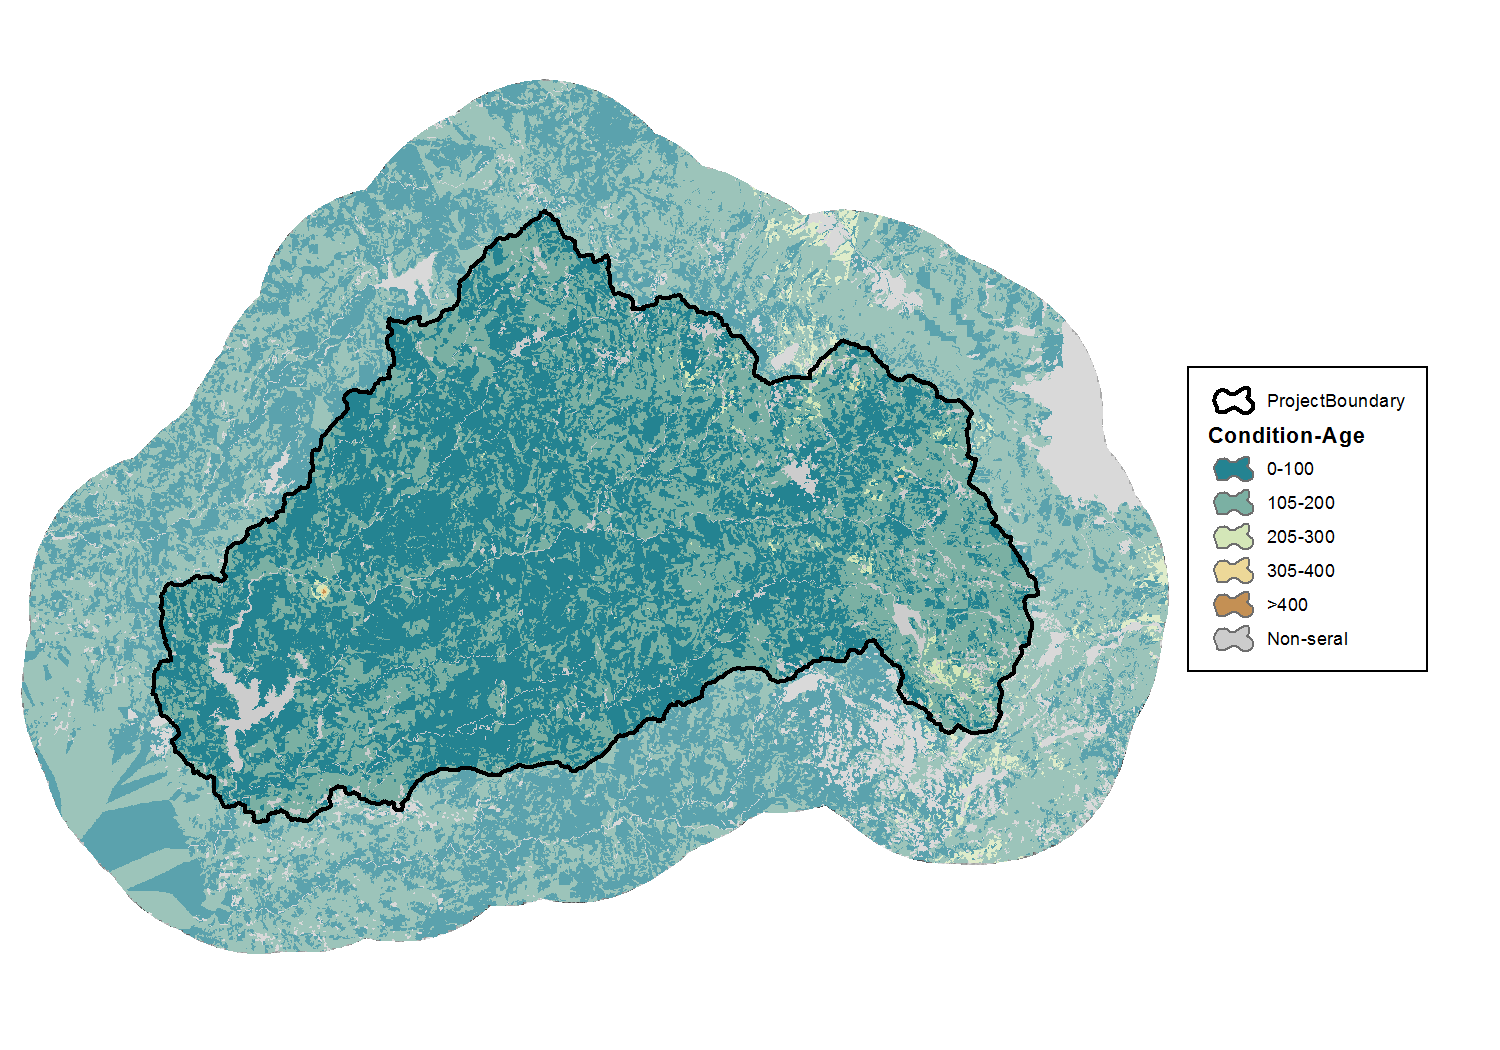
\includegraphics[height=0.4\textheight]{/Users/mmallek/Tahoe/Report2/images/condage.png}
\caption{Condition-Age map at Timestep 0 for the project area. Also shows the 10 km buffer from the project area boundary.} 
\label{condagemap}
\end{figure}

\subsubsection{Topographic Position Index}
Our topographic position index (TPI) combines heat load, which is based on aspect and slope, with slope position (Figure~\ref{tpimap}). High values for TPI are correlated with locations on steep, south and west-facing, upper slopes. Low values are correlated with locations on gentle, north and east-facing, valley bottoms. Values in between occur along a gradient of these characteristics. The TPI is scaled to the project area and the region immediately surrounding it, and is therefore a local index only. We use TPI to adjust vegetation susceptibility and mortality because we expect susceptibility and mortality to be higher when TPI is high.

\begin{figure}[htbp]
\centering
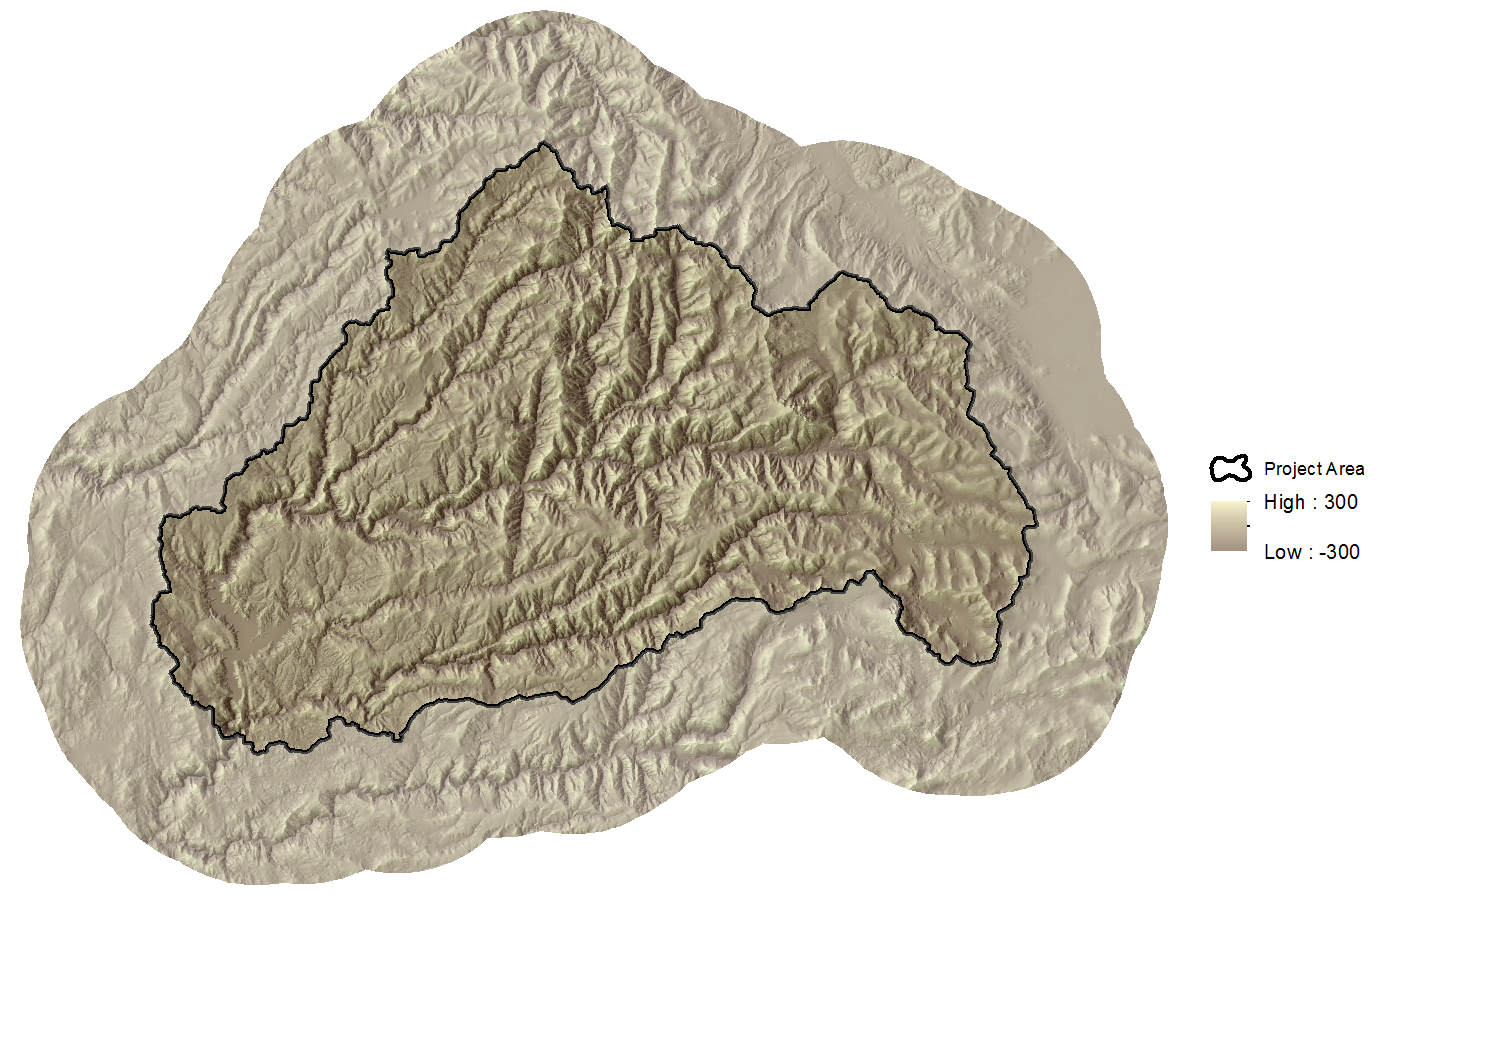
\includegraphics[height=0.4\textheight]{/Users/mmallek/Tahoe/Report2/images/tpi.png}
\caption{Topographic Position Index for the project area. Also shows the 10 km buffer from the project area boundary.} 
\label{tpimap}
\end{figure}

\subsubsection{Elevation} 
Elevation represents the height above sea level in meters. Elevation is typically derived from an existing digital elevation model (DEM). In \textsc{RMLands}, the elevation layer affects disturbance spread. \todo{Correct?} Elevation is a \emph{static} grid; cell values remain constant over time. The elevation grid used in this analysis was provided by the Tahoe National Forest GIS staff and rescaled from 10 m$^2$ to 30 m$^2$ pixels. It is shown as a map in Figure~\ref{elevationmap}.

\begin{figure}[htbp]
\centering
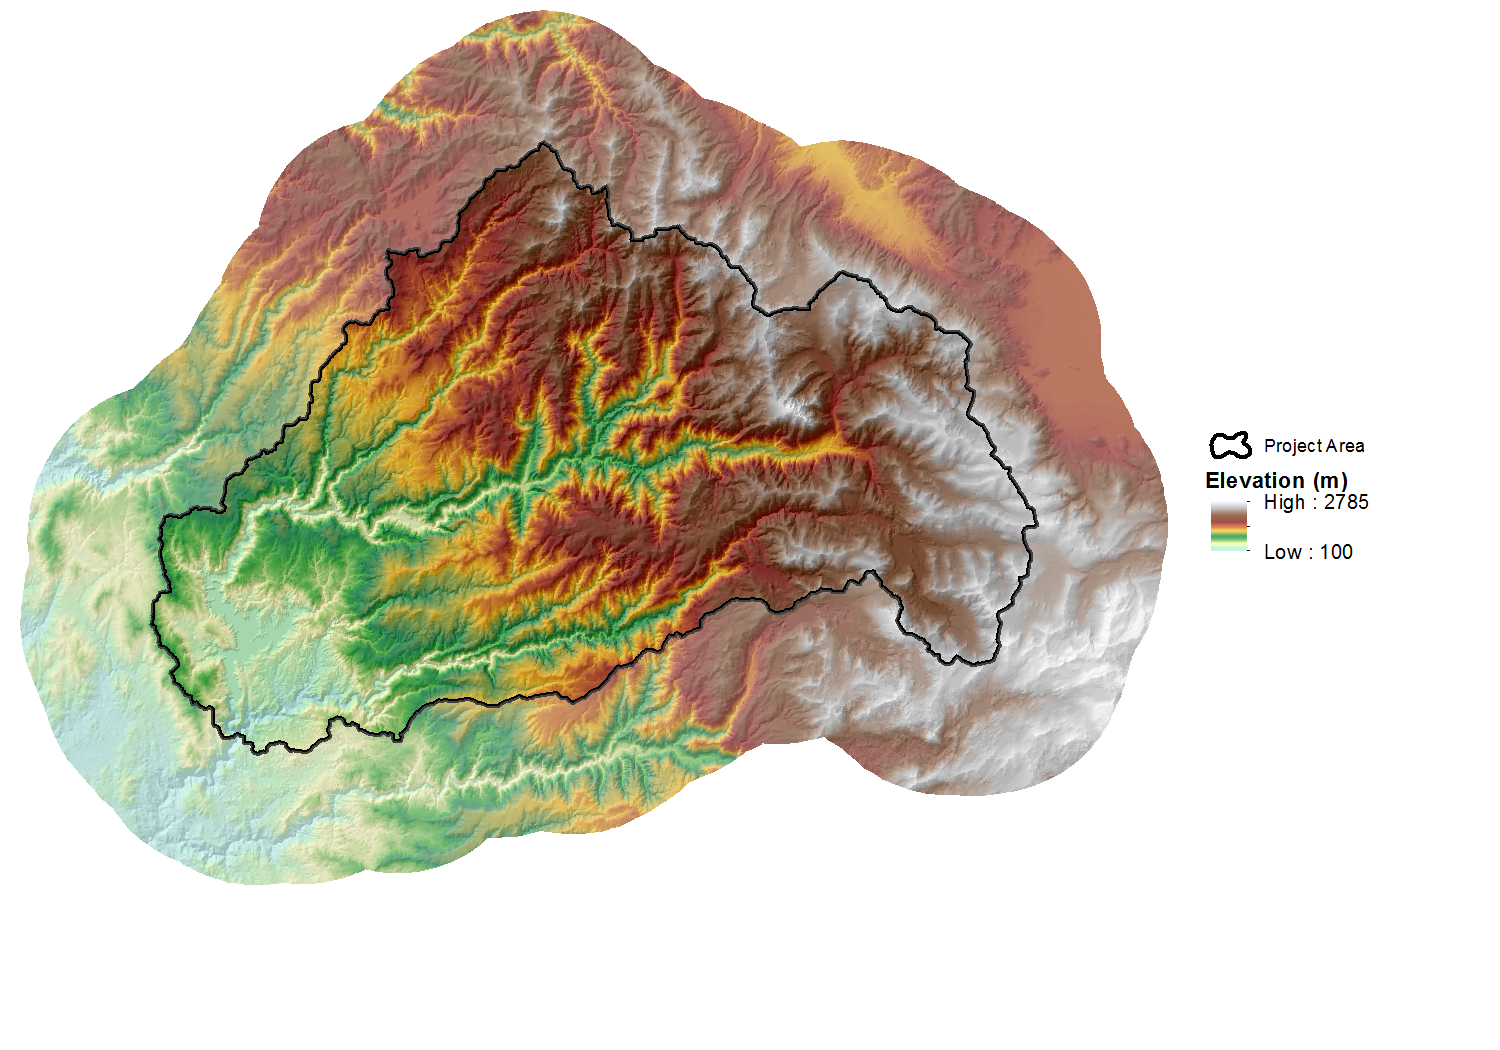
\includegraphics[height=0.4\textheight]{/Users/mmallek/Tahoe/Report2/images/elevation.png}
\caption{Elevation for the project area. Also shows the 10 km buffer from the project area boundary.} 
\label{elevationmap}
\end{figure}

\subsubsection{Slope} 
Slope represents the steepness of a cell as measured in percent and is derived from the elevation layer. Slope is used in GIS preprocessing to define cover types and eligibility for various vegetation treatments. Within \textsc{RMLands}, slope affects disturbance spread. Slope is a \emph{static} grid; cell values remain constant over time. The slope for the study area is shown in Figure~\ref{slopemap}.

\begin{figure}[htbp]
\centering
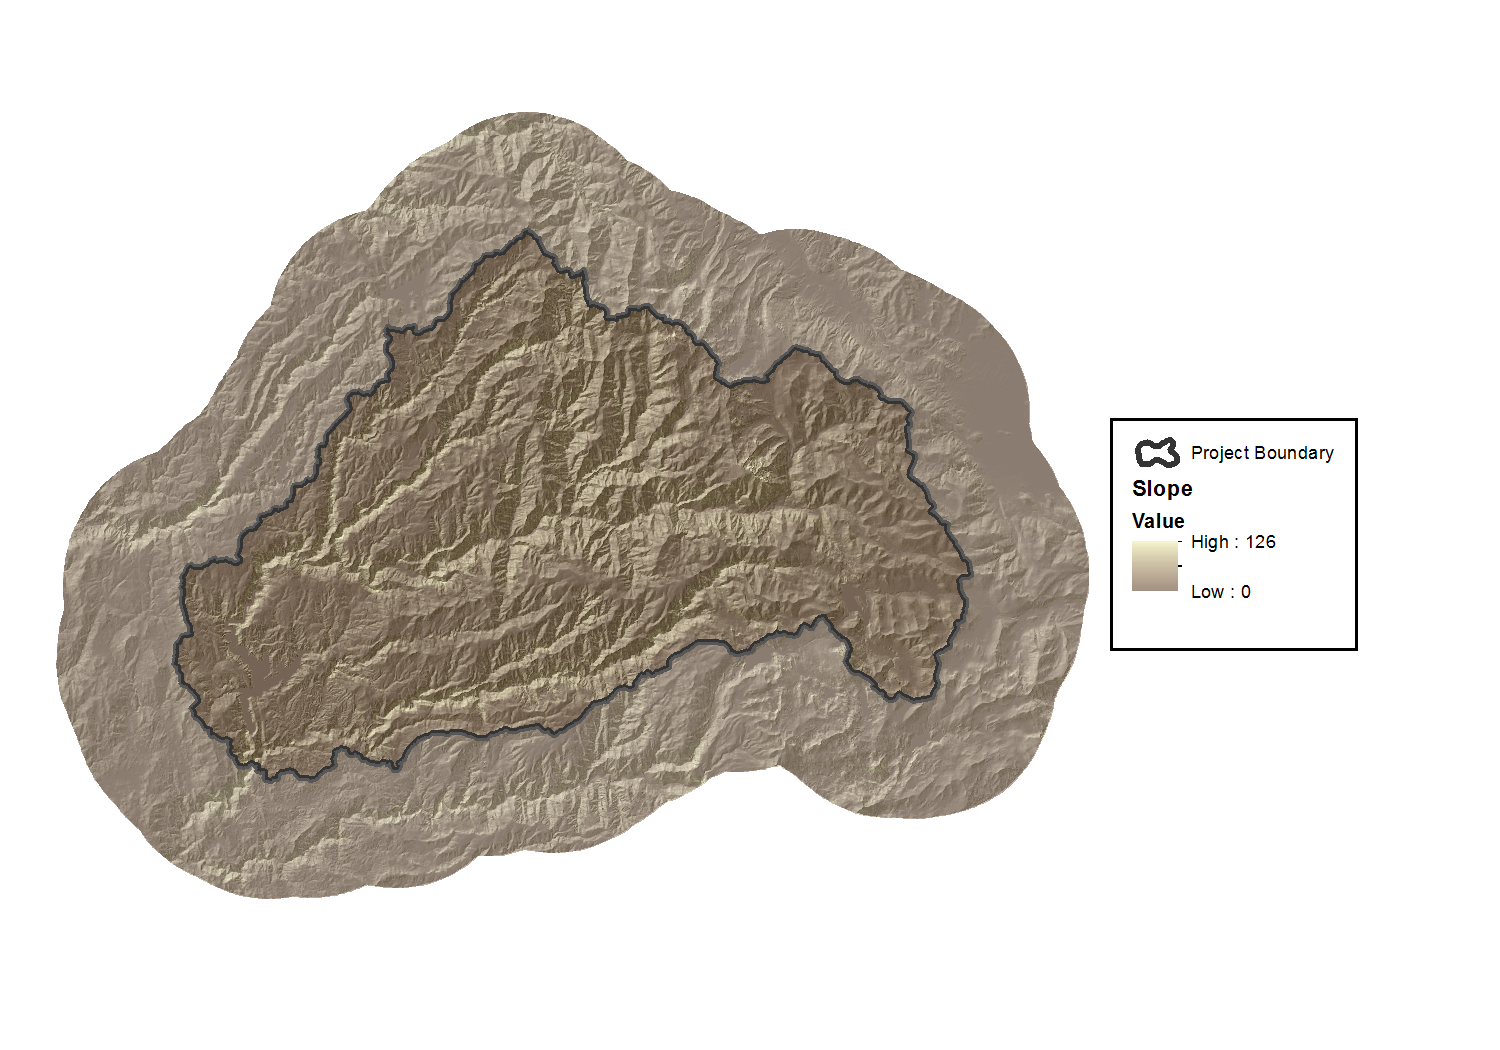
\includegraphics[height=0.4\textheight]{/Users/mmallek/Tahoe/Report2/images/slope.png}
\caption{Slope for the project area, which ranges from flat to 126\%. Also shows the 10 km buffer from the project area boundary.} 
\label{slopemap}
\end{figure}

\subsubsection{Aspect} Aspect represents the direction that a cell faces and is derived from elevation. It primarily affects the spread of disturbance in \textsc{RMLands}. Aspect is a \emph{static} grid; cell values remain constant over time. Grid values represent categorical values assigned to the eight cardinal directions, plus a value for flat areas with no aspect (see Figure~\ref{aspectmap}. 

\begin{figure}[htbp]
\centering
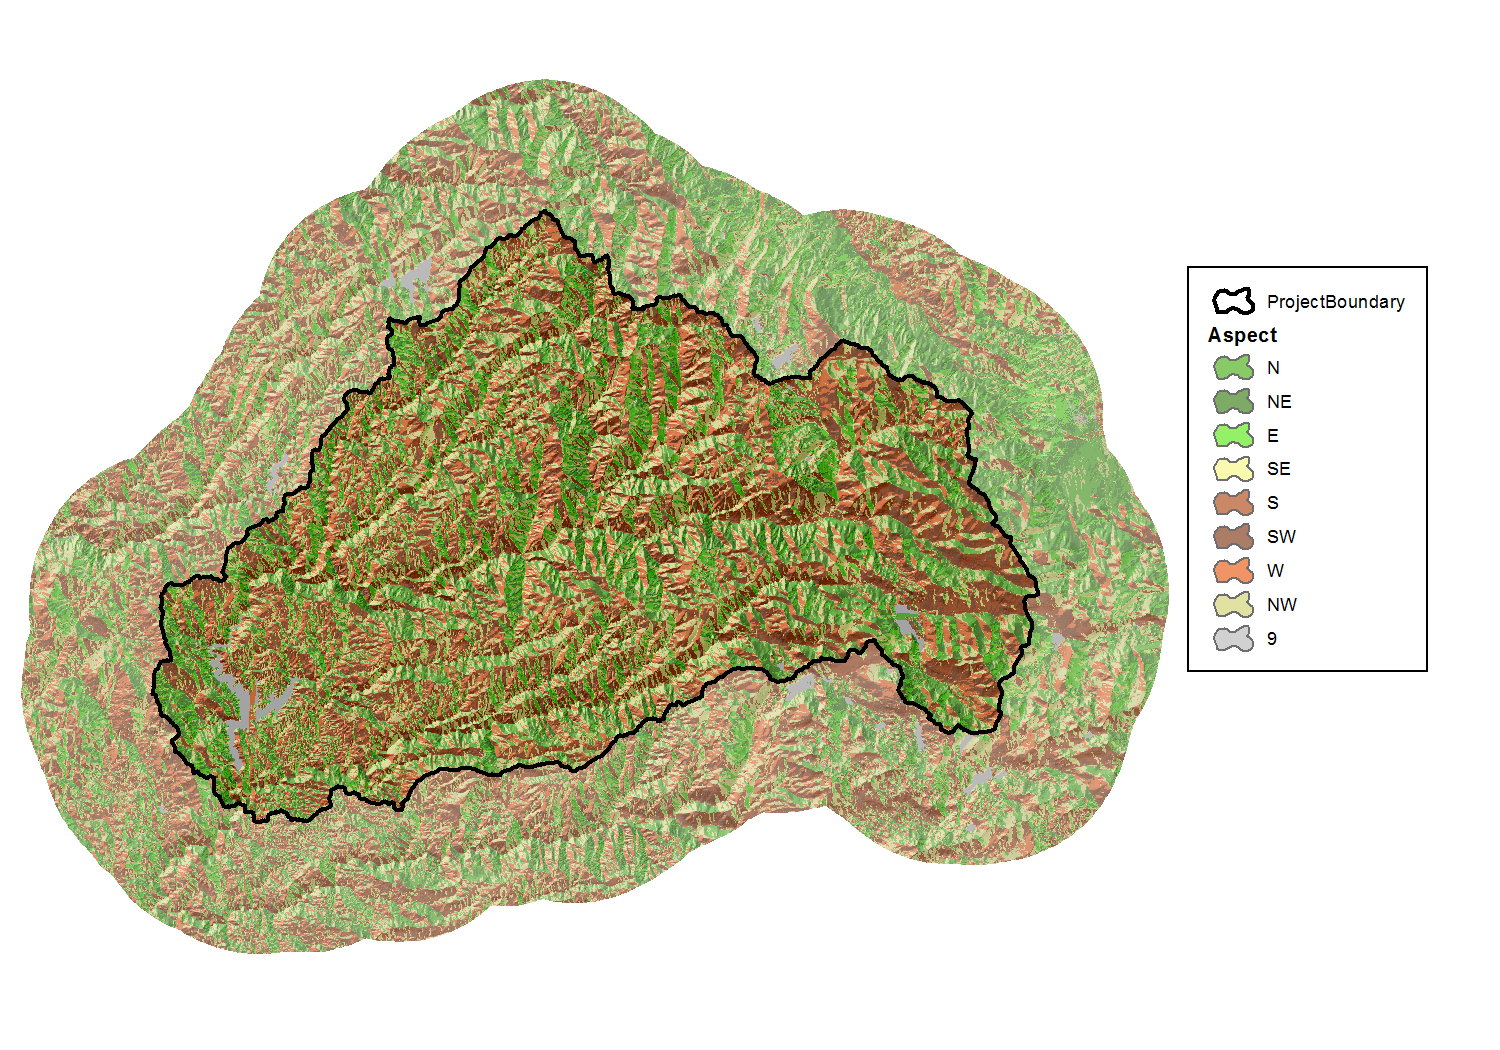
\includegraphics[height=0.4\textheight]{/Users/mmallek/Tahoe/Report2/images/aspect.png}
\caption{Aspect for the project area. Also shows the 10 km buffer from the project area boundary.} 
\label{aspectmap}
\end{figure}

\subsubsection{Streams} 
Streams represents aquatic communities classified as small, medium or large based on stream order. In this application, the streams layer was created from a line coverage containing hydrography data, including an attribute for stream size or order, by converting to a grid based on the stream size attribute. Streams are a potential barrier to the spread of wildfire disturbance in \textsc{RMLands}, or may be used as a natural boundary to a treatment unit, depending on their size.

We employed the orthogonal neighbor rule when converting a line to a raster of like-valued cells. That is, the final grid contains stream cells that connect along a cell side, as opposed to diagonally. This is required because diagonal neighbors, while touching, will not provide an impediment to disturbance spread (which happens diagonally as well as orthogonally). In addition, streams did not have to be in a contiguous network, which has implications in terms of disturbance spread and/or logical treatment boundaries; in general breaks in the stream network happens only near stream headwaters. 

Streams is a \emph{static} grid; cell values remain constant over time. Note, streams are integrated into the cover type classification scheme insofar as they are classified as type ``Water'' in the Existing Vegetation Layer. Regardless, they also exist as a single layer. Grid values represent categorical values assigned to the three stream size classes, plus a value for background. The final streams input layer is shown in Figure~\ref{streamsmap}.

\begin{figure}[htbp]
\centering
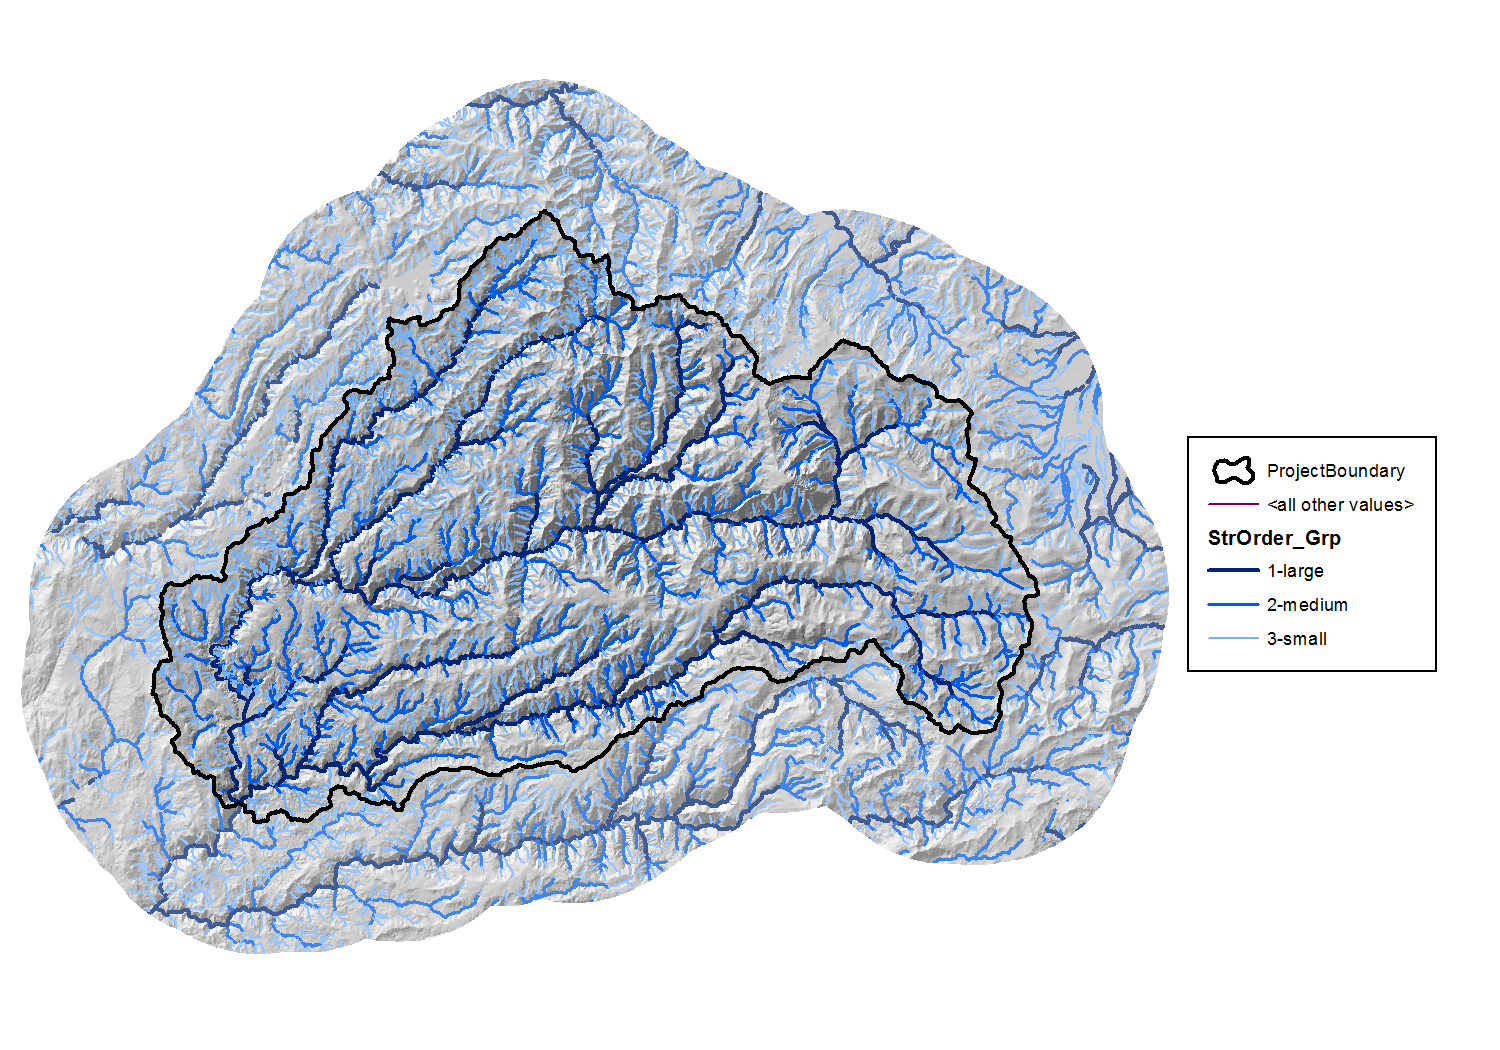
\includegraphics[height=0.4\textheight]{/Users/mmallek/Tahoe/Report2/images/streams.png}
\caption{Streams in the project area. Also shows the 10 km buffer from the project area boundary.} 
\label{streamsmap}
\end{figure}

\subsubsection{Buffer/Core} 
Buffer is a grid where the ``core'' project area is represented by one integer value, while its ``buffer'' around the core area is represented by a second integer value. The ``core'' area is the project area of interest (the watersheds), whereas the ``buffer'' is an arbitrarily-defined area around the core designed to eliminate the boundary (or edge) effect associated with disturbance spread. This allows disturbances to spread on to and off of the landscape without impediment. Without a buffer there is a substantial bias in the probability of disturbance for cells within a certain distance of the edge of the landscape because of the reduced likelihood that disturbances will spread to that location from outside the designated landscape. We use a 10 km buffer, which is generally sufficient to offset any boundary effects when simulating large wildfires. Because a buffer grid is specified, all other input grids must be classified within the full extent of the buffer area as well as the core. All succession and disturbance processes operate seamlessly across the buffer and core, and thus the presence of the buffer does not affect the simulation in any way. However, with the buffer present, all statistical reporting is restricted to the behavior in the core only. Buffer is a \emph{static} grid; cell values remain constant over time. The original polygon layer for this was generated by creating at 10km buffer around the project area watersheds. It was then converted to raster using the same procedure as for other layers. The buffer and core are easily distinguished in Figures~\ref{covermap}--\ref{streamsmap}: the core is the interior area delinated by a thick black line, while the buffer is area outside of this line, displayed at a decreased brightness level.



\subsection{Model Parameterization}
\label{subsec:hrvmodelparam}

\subsubsection{State and Transition Models}
We have created a detailed cover type description document for each cover type in the simulated landscape that experiences transitions between cover class. These documents describe crosswalks to other data layers, detailed accounts of the multiple species characteristic of the cover type, cover type distribution, relationship and response to wildfire, predicted fire return intervals, plus descriptions of each condition class present within the cover type and their succession and wildfire transition conditions and rates. \todo{APPENDIX?} Each detailed document can be summarized as a state and transition model for a particular cover type, which is implemented in the model by specifying susceptibility to wildfire, rules for vegetational succession, and rules for transitions after a fire event. Figure~\ref{transmodel} shows a generic example state and transition model for the forested cover types.

\begin{figure}[htbp]
\centering
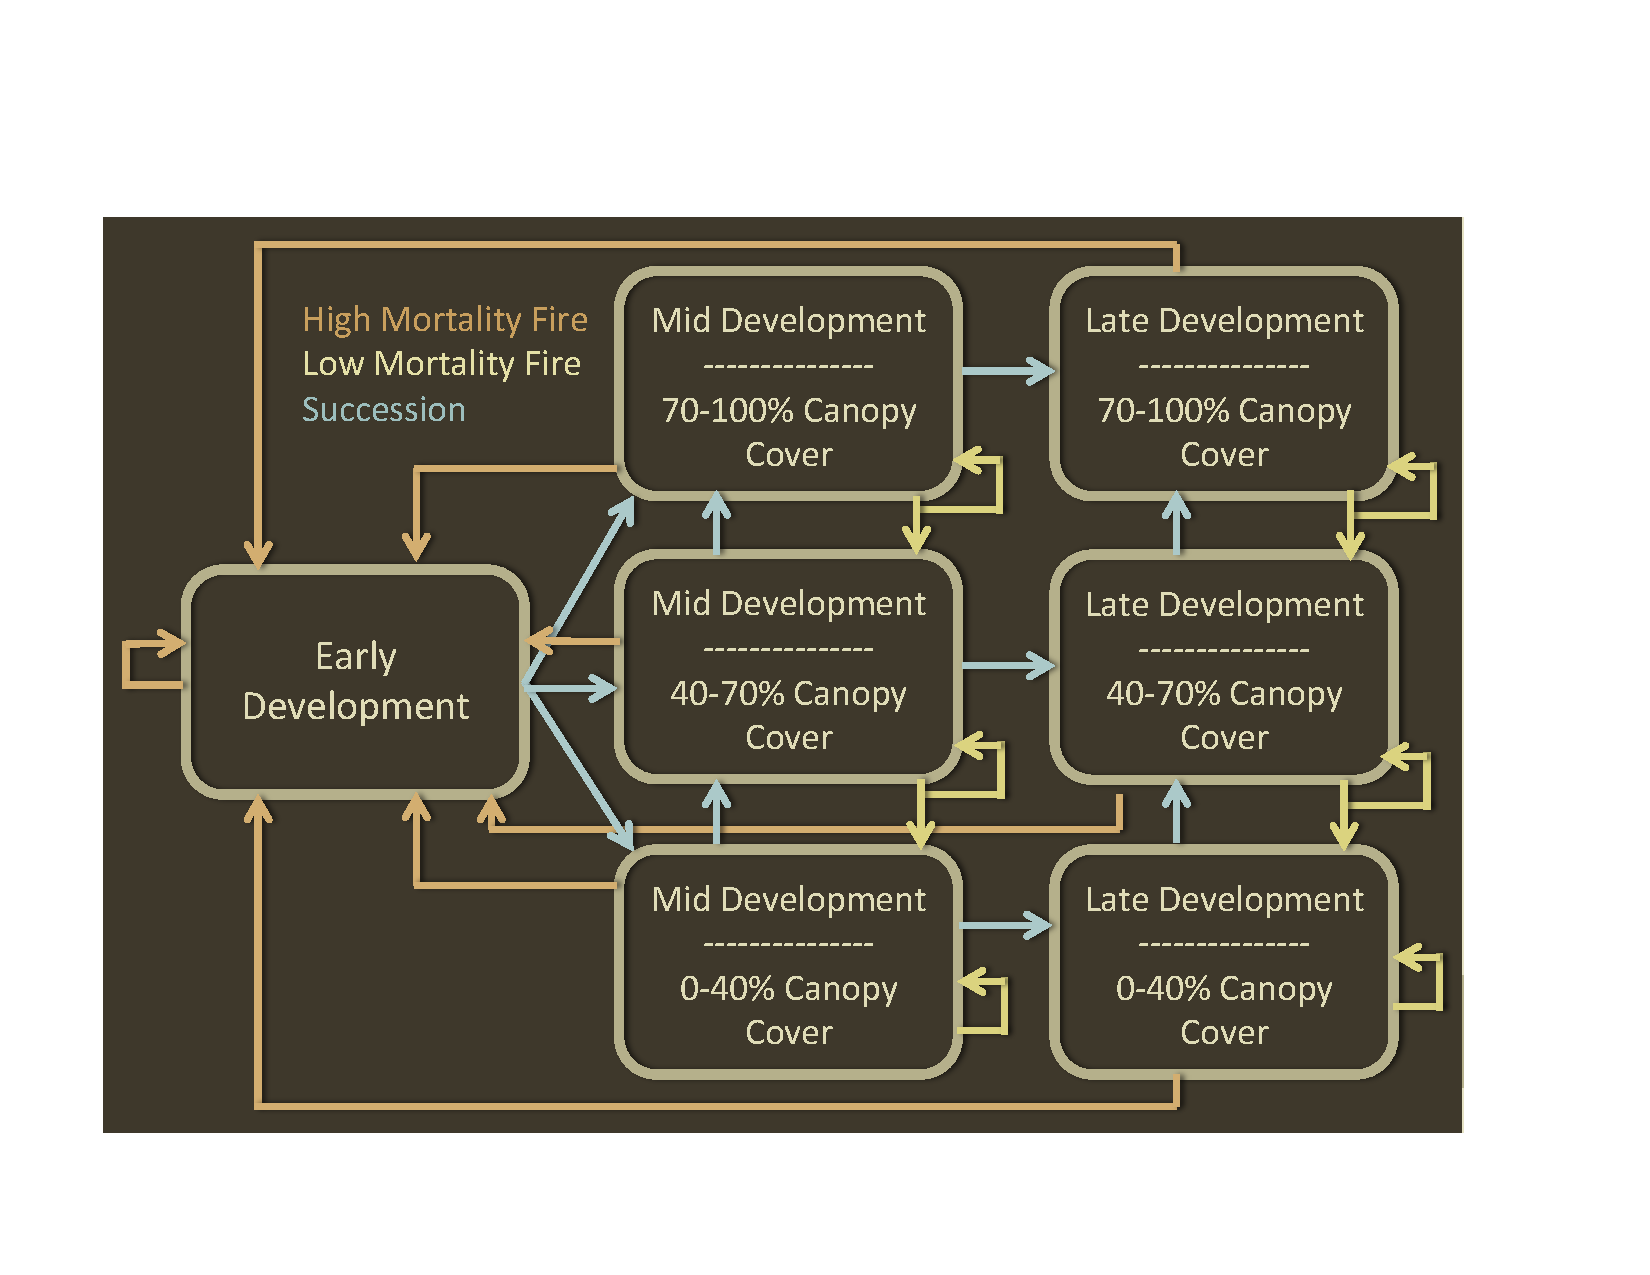
\includegraphics[width=0.8\textwidth]{/Users/mmallek/Tahoe/Report2/images/STModel_PowerPoint.pdf}
\caption{Generic state and transition model for all non-shrub seral cover types. Boxes show seven condition classes and arrows depict transitions due to vegetation succession and high or low mortality fire.} 
\label{transmodel}
\end{figure}

To illustrate the parameterization, in the following tables we present values for the Sierran Mixed Conifer - Mesic cover type model. The target fire return interval for this cover type is 29 years. Specific FRIs and probabilities of high mortality fire are specified for each condition class (Table~\ref{smcm_fri_phm}). In addition, we specified transition probabilities for natural succession between the early, middle, and late stages of development, as well as between closed, moderate, and open canopy cover. This type of succession also depends on the \emph{Condition-Age} or \emph{Stage-Age}\footnote{Stage-Age is not an input layer to \textsc{RMLands}; it is created on-the-fly.} of a particular cell (Table~\ref{smcm_vegtrans}). Finally, probabilities are specified for vegetation transitions after wildfire (Table~\ref{smcm_firetrans}). We calculated these values using the VDDT models associated with the LandFire project, modifying some based on local expert opinion. From the VDDT models, we used the probabilities of a transition to early seral conditions, a more open canopy condition, or of no transition. We ignored the classified type of fire (as replacement, mixed, or low severity), focusing instead on the outcome from fire in terms of the condition, if any, to which a cell transitioned after wildfire.


\begin{table}[htbp]
\small
\centering
\caption{Fire return interval and percent high mortality fire probabilities for Sierran Mixed Conifer - Mesic.}
\label{smcm_fri_phm}
\begin{tabular}{lcc}
\hline
\textbf{Condition Class}    & \textbf{FRI (yrs)} & \textbf{\% High Mortality} \\ \hline
\emph{Target}    			& \emph{29}&                   \\
Early All     				& 44        & 1                 \\
Mid Closed    				& 19        & 0.23              \\
Mid Moderate  				& 13        & 0.17              \\
Mid Open      				& 10        & 0.14              \\
Late Closed   				& 34        & 0.37              \\
Late Moderate 				& 13        & 0.14              \\
Late Open     				& 8         & 0.09              \\ \hline
\end{tabular}

\end{table}

\begin{table}[!htbp]
\small
\centering
\caption{Timeframes for transitions between condition classes in \textsc{RMLands} for Sierran Mixed Conifer - Mesic. ``Early to Mid'' and ``Mid to Late'' times are based on the time in a developmental stage, regardless of disturbance history. ``Open to Moderate'' and ``Moderate to Closed'' times are based on the time in a condition class since a disturbance.}
\label{smcm_vegtrans}
\begin{tabular}{cccc}
\hline
\textbf{Condition Class Transition} & \textbf{Minimum (years)} & \textbf{Average (years)} & \textbf{Maximum (years)} \\ \hline
Early to Mid 	& 20      & 26      & 40      \\
Mid to Late 	& 100     & 113     & 150     \\
\begin{tabular}[c]{@{}c@{}}Open to Moderate or\\ Moderate to Closed\end{tabular}  & 15      & 21      &    ---     \\ \hline
\end{tabular}

\end{table}


\begin{table}[!htbp]
\small
\centering
\caption{Transition probabilities for Sierran Mixed Conifer - Mesic following low mortality fire.}
\label{smcm_firetrans}
\begin{tabular}{lcc}
\hline
\textbf{Condition Class Transition} & \textbf{Probability}\\
\hline
Mid Closed to Mid Moderate     	& 0.5263   	\\
Mid Moderate to Mid Open    	& 0.357		\\
Late Closed to Late Moderate	& 0.5435    \\
Late Moderate to Late Open     	& 0.2442    \\
\hline
\end{tabular}
\end{table}

Transitions between Early and Middle Development, and between Middle and Late Development are governed by the time in the Early or Middle stage (canopy cover usually does not affect these probabilties). These transitions may begin at the minimum time in a developmental \emph{stage} specified, and proceed at rates that vary across cover types. Figure~\ref{smcm_vegtrans} displays the average \emph{Stage-Age} of transition. If a cell reaches the maximum stage-age listed, its probability of transitioning goes to 1. Transitions between the canopy cover types occur within one developmental stage: e.g., between Middle Development Open and Middle Development Moderate, but not between Middle Development Open and Late Development Moderate. These transitions are governed by the time in the full condition class specification since the last disturbance. This ``years since'' value may be affected by a low mortality fire, a transition between developmental stages, or a transition between canopy cover levels. Similarly to the developmental transitions, the shift from, for example, Middle Development Open to Middle Development Closed may begin when the minimum time is reached, and also proceeds at rates that vary across cover types. Figure~\ref{smcm_vegtrans} shows the average condition-age of transition. However, no maximum age is specified for this type of transition.

\subsubsection{Disturbance Parameters} 
\label{subsubsec:distparams}

%\begin{adjustwidth}{5ex}{0pt}
\begin{itemize}
\item \emph{Climate:} The climate parameters are based on a rescaling of the Palmer Drought Severity Index (PDSI). PDSI is a long-term measure of drought, on the scale of months to years. It is based on precipitation and temperature and incorporates soil moisture. Resconstructed PDSI values for summer months during the historic period of this project (1550-1850) are available from Zhang 2004, Zhang 2009, and Cook 2004. These data are summarized at large scales; for example, the Cook 2004 data are calculated for a grid with points spaced at 2.5\textdegree. We selected the five closest points to the center of the project area from the Cook and Zhang datasets and calculated the inverse distance-weighted mean of the values. We then converted the yearly data into five-year averages to align with the five-year timesteps in our model. By recentering the mean value around 1 and then taking the inverse, we create a dataset in which a value of 1 is neither wetter nor dryer than average, values between 0 and 1 represent wetter-than-normal timesteps, and values greater than 1 represent dryer-than-normal timesteps (Figure~\ref{pdsi}). Climate interacts with other disturbance parameters in \textsc{RMLands}, including initiation, susceptibility, and spread.

\begin{figure}[htbp]
\centering
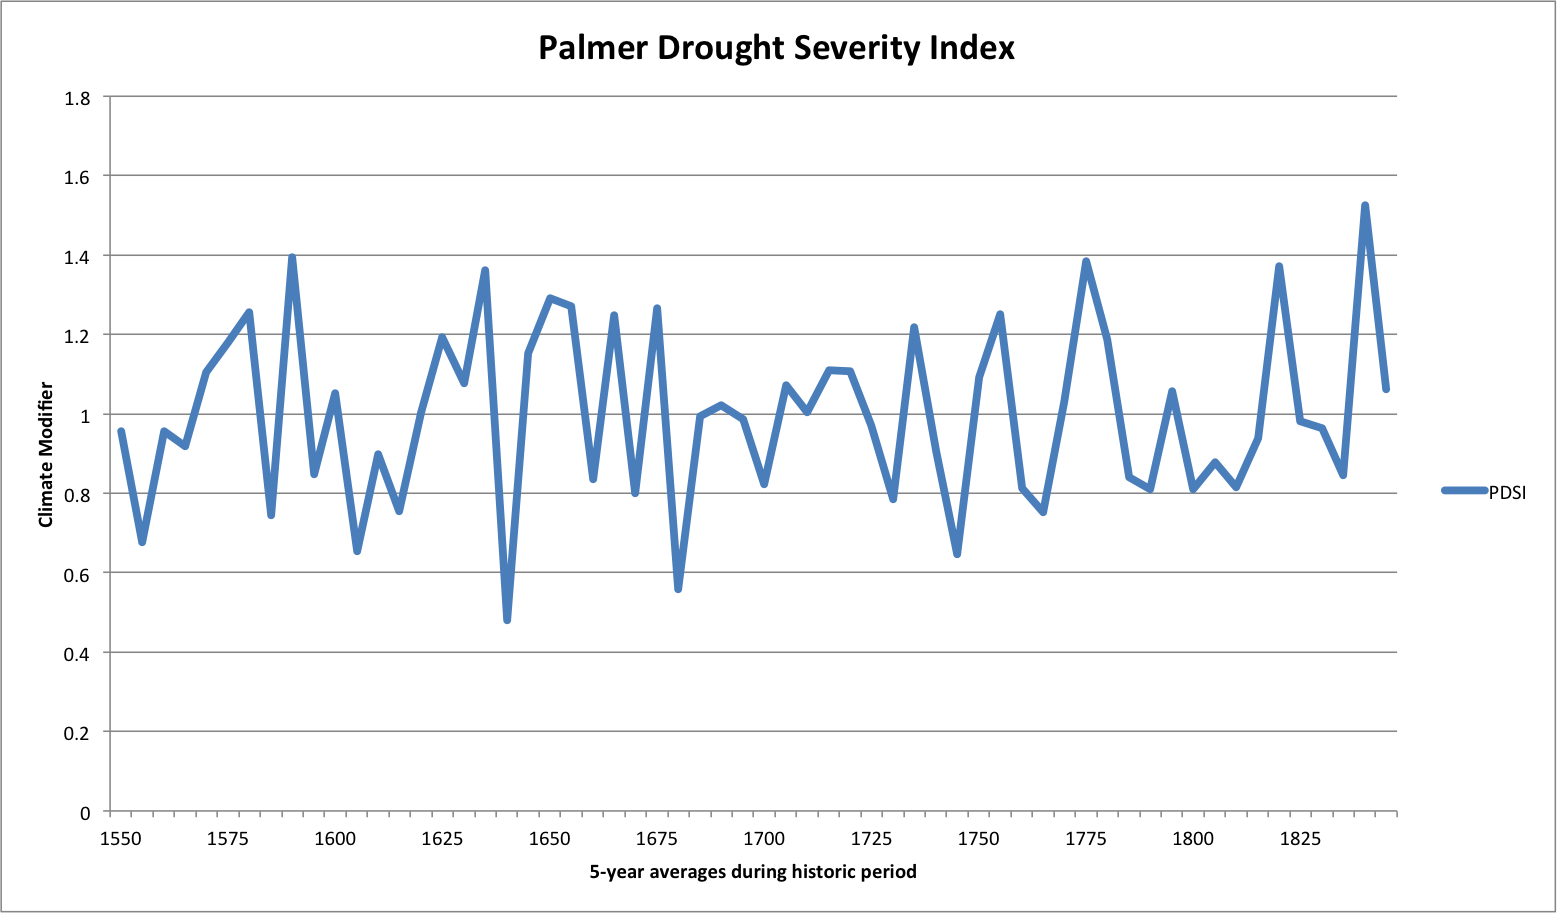
\includegraphics[height=0.3\textheight]{/Users/mmallek/Tahoe/Report2/images/pdsi.png}
\caption{Palmer Drought Severity Index, rescaled, inverted, and presented as a 5-year average for the ``historic'' period in this study (1550-1850).} 
\label{pdsi}
\end{figure}

%\medskip

%\noindent 
\item \emph{Susceptibility:} Cover and condition are both inputs to susceptibility. Cover modifies susceptibility via the ability to specify the influence of TPI on susceptibility (Table~\ref{covtpi}. The magnitude of this effect is estimated as a potential reduction in susceptibility of 30\% between the minimum and maximum TPI values used in the model. This is specified as part of a 4-parameter logistic function in which the left value is 0.7, right value is 1, slope is 1, and inflection point is 0.\todo{Are there typical symbols for these parameters we could use instead of right and left?} 

\begin{table}[htbp]
\small
\centering
\caption{Cover types whose susceptibility is modified by Topographic Position Index.}
\label{covtpi}
\begin{tabular}{ll}
\hline
\multicolumn{2}{c}{\textbf{Cover Types with TPI Adjustment}} \\
\hline
Grassland     									& Red Fir - Mesic   					\\
Lodgepole Pine    								& Red Fir - Ultramafic					\\
Mixed Evergreen - Mesic							& Red Fir - Xeric    					\\
Mixed Evergreen - Ultramafic     				& Sierran Mixed Conifer - Mesic    		\\
Mixed Evergreen - Xeric 						& Sierran Mixed Conifer - Ultramafic 	\\
Montane Riparian								& Sierran Mixed Conifer - Xeric 		\\
Oak Woodland 									& Western White Pine					\\
Oak-Conifer Forest and Woodland 				& Yellow Pine 							\\
Oak-Conifer Forest and Woodland - Ultramafic 	&										\\
\hline
\end{tabular}

\end{table}

Condition class further modifies susceptibility. We use the Weibull cumulative distribution function and specify a scale parameter $\lambda$ (mean return interval), shape parameter $k$, and the reset point for the function (\emph{age since high mortality disturbance} or \emph{age since any disturbance}). The mean return interval for the condition class is used as a calibration parameter and was initially set as equal to the values provided in analogous LandFire Biophysical Setting types.\todo{cite} Some modifications were made based on consultation with Forest Service staff. All mean return intervals within a cover type are modified as a group and kept relative to one another even as the magnitude of the return intervals is adjusted. We set $k=3$ for all cover types and condition classes. We selected between ``age since high mortality disturbance'' and ``age since any disturbance'' based on whether wildfires in that cover type are climate-driven (in which case we select the former) or fuels-driven (in which case we select the latter) (Figure~\ref{howdriven}). A detailed description of the specific parameters chosen is available \todo{in some sort of appendix type file, or perhaps in cover type description doc?}.

\begin{table}[htbp]
\small
\centering
\caption{Cover types sorted by whether wildfire disturbance in them is characterized by fuels present or overarching climatic conditions. If the likelihood of wildfire depends on the accumulation of fuels, the value of $x$ (``time since'') reverts to 0 after any disturbance. If the likelihood of wildfire depends primarily on climate and weather conditions, the value of $x$ reverts to 0 only after a high mortality disturbance.}
\label{howdriven}
\begin{tabular}{ll}
\hline
\textbf{Fuel-Driven Cover Types} 				& \textbf{Climate-Driven Cover Types}	\\
\hline
Curl-leaf Mountain Mahogany 					& Agriculture   						\\
Grassland     									& Big Sagebrush 						\\
Lodgepole Pine    								& Black and Low Sagebrush				\\
Meadow											& Lodgepole Pine with Aspen 			\\
Mixed Evergreen - Mesic							& Montane Riparian						\\
Mixed Evergreen - Ultramafic     				& Red Fir with Aspen   					\\
Mixed Evergreen - Xeric 						& Red Fir - Mesic    					\\
Oak Woodland 									& Red Fir - Ultramafic 					\\
Oak-Conifer Forest and Woodland 				& Red Fir - Xeric 						\\ 	
Oak-Conifer Forest and Woodland - Ultramafic 	& Subalpine Conifer 					\\
Sierran Mixed Conifer - Ultramafic 				& Subalpine Conifer with Aspen 			\\
Sierran Mixed Conifer - Xeric 					& Sierran Mixed Conifer with Aspen 		\\
Urban 											& Sierran Mixed Conifer - Mesic 		\\
Yellow Pine 									& Western White Pine 					\\
												& Yellow Pine with Aspen 				\\
\hline
\end{tabular}
\end{table}


%\medskip

%\noindent 
\item \emph{Initiation:} In \textsc{RMLands}, parameters for initiation are used as calibration parameters. The probability of wildfire initiation is a function of its susceptibility to wildfire and the climate modifier value for that timestep, and is applied at the cell level. The ignition calibration coefficient refers to the number of ignitions per 100,000 ha per year. For the HRV simulation, we set this coefficient at 38. We applied the coefficient evenly across the landscape based on local expert knowledge of lighting strike locations in the area (Alan Doerr and Marilyn Tierney, personal communication). Fires may be initiated anywhere within the project area or the 10 km buffer around it. The total area cover within that boundary is 409,410.7 ha, so up to 777 fire starts were possible during each timestep in our simulation (not all potential ignitions result in fire). Climate also influences initiation.

%\medskip

%\noindent 
\item \emph{Spread:} The probability of fire spread in \textsc{RMLands} is a function of climate, susceptibility to wildfire, potential wildfire size, wind, spotting, relative elevation, and presence of streams. The first two are described above. The disturbance size distribution that regulates potential fire size was created by analyzing the size distribution of all mapped fires in the Northern Sierra CalVeg mapping zone and west of the Sierran crest, available from the Forest Service and the California Department of Forestry and Fire Protection, which goes back to approximately 1900. 

Wind is incorporated in two parts. First, a prevailing wind direction for the fire is selected probabilistically from the eight cardinal directions. To compute the wind distribution values, we first consulted local experts to determine the dates of fire season (May 15 to October 15) and burning period times (1000 hours to 1800 hours). We then downloaded all available historic wind direction data from 6 local weather stations (Rice Canyon, Saddleback, Downieville, White Cloud, Emigrant Gap, and Blue Canyon, Figure~\ref{weather}). Data from all weather stations was weighted equally. After the wind direction is selected, fires are able to grow in all directions, but are relatively more likely to spread with wind than against it. We parameterized the influence of \emph{relative wind} as a reduction in spread likelihood. Thus, spread in the same direction as wind has a neutral effect, spread at $\ang{45}$ angles is reduced by 30\%, spread at $\ang{90}$  angles is reduced by 70\%, spread at $\ang{135}$ angles is reduced by 90\%, and spread opposite the prevailing wind direction is reduced by 95\%. 

\begin{figure}[htbp]
\centering
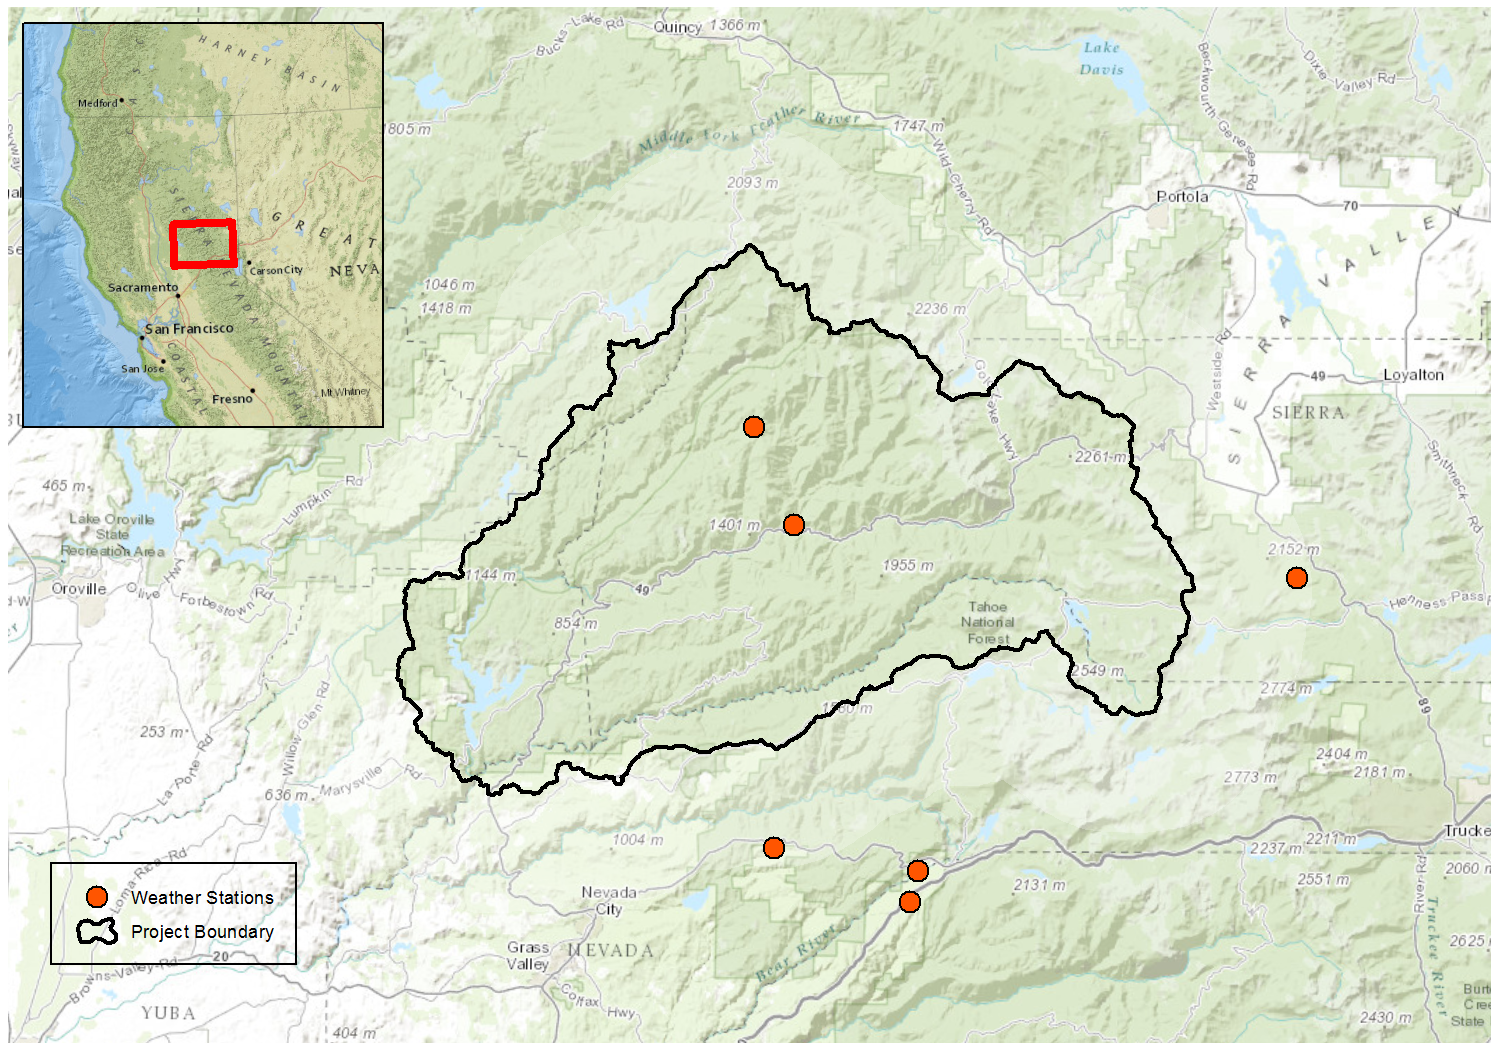
\includegraphics[width=0.8\textwidth]{/Users/mmallek/Tahoe/Report2/images/weather.png}
\caption{Weather stations used to inform wind direction parameters.}
\label{weather}
\end{figure}

Relative elevation also modifies spreading potential. We parameterized the model such that spread downhill is extremely unlikely. Spotting and the extent to which streams act as barriers to spread are affected by the fire size. As fires become larger, their probability of spotting and spotting distance increases. Similarly, streams function as a barrier to smaller fires, but large fires are able to spread past streams regardless of size. This decision is based on the idea that large fires are more influenced by wind and climatic conditions. Stream size does impact smaller fires; the largest streams and rivers are usually an effective barrier to smaller fires, although even fairly small fires often spread past intermittent and small perennial streams. 

For complete precise parameterization of the model, see \todo{Where would this go? Screenshots or table?}


\item \emph{Mortality:} Cover and condition are both inputs to mortality. The effect of topographic position is tied to cover: the mortality of certain cover types (Table~\ref{covtpi}) is affected by cover. The magnitude of this effect is estimated as a potential reduction in mortality of 30\% between the minimum and maximum TPI values used in the model. This is specified as part of a 4-parameter logistic function in which the left value is 0.7, right value is 1, slope is 1, and inflection point is 0. \todo{same issue - would be better to state greek letters instead of right/left.}

\begin{table}[htbp]
\small
\centering
\caption{Cover types whose mortality is modified by Topographic Position Index.}
\begin{tabular}{ll}
\hline
\multicolumn{2}{c}{\textbf{Cover Types with TPI Adjustment}} \\
\hline
Grassland     									& Red Fir - Mesic   					\\
Lodgepole Pine    								& Red Fir - Ultramafic					\\
Mixed Evergreen - Mesic							& Red Fir - Xeric    					\\
Mixed Evergreen - Ultramafic     				& Sierran Mixed Conifer - Mesic    		\\
Mixed Evergreen - Xeric 						& Sierran Mixed Conifer - Ultramafic 	\\
Montane Riparian								& Sierran Mixed Conifer - Xeric 		\\
Oak Woodland 									& Western White Pine					\\
Oak-Conifer Forest and Woodland 				& Yellow Pine 							\\
Oak-Conifer Forest and Woodland - Ultramafic 	&										\\
\hline
\end{tabular}
\end{table}

Condition class further modifies mortality. We extracted the likelihood of mortality from the VDDT models built during the LandFire project. However, our accounting method differs slightly. VDDT characterizes fire severity (e.g. mixed) independently from a particular outcome (e.g. resetting to early seral conditions). We do not include ``mixed severity'' fire in our model. Instead, we characterize fire dichotomously, based on their outcomes: fires are either high mortality or low mortality events. We define low mortality fires are those in which less than 70\% of overstory trees are killed, while high mortality fires are those in which more that 70\% of overstory trees are killed. 

To interpret the VDDT models, we analyzed not only the fire type (replacement, mixed, or surface), but also the change in \emph{condition} that occurred as a consequence of that fire. I classified the probabilities specified by the VDDT model as associated with either high or low mortality fires. High mortality fires are those that result in conversion to early seral (regardless of whether they are called ``replacement'' or ``mixed''). All other fires are considered low mortality. The probability of a high mortality outcome from fire was calculated by dividing the summed probabilities of high mortality fires as defined above by the summed probabilities of all fires. As an example, these probabilities for Sierran Mixed Conifer - Mesic are provided in Table~\ref{smcm_fri_phm} (Subsection~\ref{subsec:hrvmodelparam}).

\end{itemize}
%\end{adjustwidth}

\subsection{Model Calibration}
Calibrating the model was done by manipulating the ignition calibration coefficient and the relative magnitude of the scale parameter (mean fire return interval) $\lambda$ in the Weibull cumulative distribution function under Susceptibility. We first manipulated the ignition calibration coefficient and reran the simulation until the output cover type rotation values were in a range near their target. We then modified the fire return interval values as groups of condition classes under a given cover type to achieve our target rotations. For example, the target rotation for Sierran Mixed Conifer - Mesic was 29 years. As part of calibration, we adjusted the input condition class-based mean fire return interval up or down, eventually arriving at an increase by a factor of 3 from the original VDDT values. That is, each scale parameter value was multiplied by 3 in order to modify the susceptibility of Sierran Mixed Conifer - Mesic to fire without changing the relative susceptibility among Sierran Mixed Conifer - Mesic condition classes. We came very close to achieving our target cover type rotation values through several iterations of this method, and the final step was to make a final small modification to the ignitition calibration coefficient.

\subsection{Model Execution}
During the calibration phase of the model, a typical simulation would be three runs of 200 timesteps each. The equilibration period of 40 timesteps was chosen based on visual analysis of the disturbed area and rotation plots from the combined runs. Once calibration was complete, we conducted one 500 timestep-long run in order to capture multiple disturbance and succession cycles across the most common cover types. Each timestep represents five years. The five-year timestep was chosen based on the short fire return intervals recorded from dendrochronology analysis in the literature and our desire to capture these very short return intervals in the simulation.

\subsection{Data Analysis}
\label{subsec:dataanalysis}

\paragraph{Disturbance Regime} We quantified the following overall temporal and spatial characteristics of the wildfire disturbance regime:
\begin{itemize}
	\item \emph{Disturbed Area:} We calculate disturbed area for each timestep, divided into low mortality and high mortality disturbance, and summed to produce an ``any mortality'' statistic. We summarize the results for minimum, maximum, mean, and median area disturbed as a proportion of the total area eligible for disturbance for the full simulation excluding the equilibration period (460 timesteps, or 2300 years). We also present maps of the landscape illustrating the minimum, maximum, and median area burned during the simulation, and a 4-timestep sequence illustrating a time series of wildfire disturbance. Finally, we present the distribution of wildfire extents during the simulation, excluding the equilibration period, as a barplot.\todo{make sure these are in the results section}
	\item \emph{Disturbance Frequency:} We calcuate the number of years between disturbances exceeding a particular threshold in total disturbed area. We report the frequency of timesteps during which at least 10\%, 25\%, or 50\% of the landscape experienced wildfire.
	\item \emph{Climate Effect:} Climate interacts with several components of the model. We present plots illustrating the change in the climate parameter by timesteps concurrently with the area disturbed per timestep. It is not practical to further illustrate its effect everywhere, and in some cases its influence is not easily separated from the other inputs to the model. \todo{be sure to make this plot} 
	\item \emph{Rotation Period:} We calculate the rotation period---the number of years required to burn an area equivalent ot the total eligible area---for each cover type within the project area. It is based on the census, not a sample, of the population of cells within the project area, and is therefore equivalent to the cell-specific grand mean return interval for a given cover type across the landscape. We report the rotation values for low mortality fire, high mortality fire, and any fire. We also report this data for the full landscape.
	\item \emph{Return Interval:} We summarize the cell-specific population mean return interval---the average number of years between disturbances at a single cell---and present it as the distribution of the percentage of eligible cells that experienced each possible mean return interval. We present histograms for low mortality fire, high mortality fire, and any fire, along with their median values. As with the rotation period, this method uses the census, not a sample, of the population of cells within the project area, and is therefore equivalent to the cell-specific grant mean return interval for a given cover type across the landscape. We also report this data for the full landscape. Finally, we present this result spatially as a map showing the population fire return interval for the full landscape and for our nine focal cover types.
\end{itemize}

\paragraph{Vegetation Response} 

\begin{itemize}
\item \emph{Landscape Composition:} We quantified the distribution and dynamics of landscape composition by cover type. For our single 2500 year simulation (with 200 year equilibration period), we summarize the results in a table and in stacked bar plots. For the tabular results, we present the mean, median, minimum, maximum, 5th, 25th, 75th and 95th percentiles of the distribution. We compared the current landscape condition (i.e., proportion of cover type in each condition class) to this simulated historic range of variability to determine whether the current landscape deviates, and to what degree, from the HRV. In the body of this report we present results for the nine focal cover types that occur over at least 1000 ha on the project landscape; others are available \todo{in an appendix? not at all?}. We visualize the proportion of the total area of a given cover type occuring as each condition class, for each timestep in the model. In addition, we show a simple plot of current conditions, allowing a visual comparison between current conditions and the historic range of variability in the distribution of the condition classes.

\item \emph{Landscape Structure and Patterns:} We used \textsc{Fragstats} \todo{cite v4.2} to compute several landscape-level and class-level metrics that summarize landscape structure over the course of the simulation. We present the results in a series of tables and figures. The descriptions below are intended as a general introduction to the \textsc{Fragstats} metrics; for a much more detailed and mathematical description of all \textsc{Fragstats} metrics, see the \href{http://www.umass.edu/landeco/research/fragstats/documents/fragstats.help.4.2.pdf}{documentation}. Each metric is computed on the study area for a single timestep and the results are displayed in tabular format by quantiles and in graphical format with line graphs.

	\begin{enumerate}
		\item Percentage of Landscape (PLAND)\\
		\emph{Landscape}-level: not computed\\
		\emph{Class}-level: the percentage of the landscape comprised of a particular patch type\\
		
		%\item Core Area Percentage of Landscape (CPLAND)\\
		%\emph{Landscape}-level: not computed\\
		%\emph{Class}-level: the sum of all core areas in a given patch type divided by the total landscape area; reported as a percentage%\\

		\item Patch Density (PD)\\
		\emph{Landscape}-level: number of patches of all cover types and condition classes divided by the total landscape area for one timestep\\
		\emph{Class}-level: number of patches of a give cover type and condition class divided by the total area occupied by that cover-condition type\\
		
		\item Edge Density (ED) \\
		\label{item:ED}
		\emph{Landscape}-level: the sum of the lengths of all edge segments divided by the total landscape area\\	
		\emph{Class}-level: the sum of the lengths of all edge segments for a given patch type divided by the total area occuring as that patch type\\

		\item Total Edge Contrast Index (TECI) \\
		\label{item:TECI}
		\emph{Note}: Contrast refers to the relative difference among patch types. For example, mature forest next to young forest might have a lower-contrast edge than mature forest adjacent to open field. A contrast weight is assigned to each possible pair of condition classes before running \textsc{Fragstats}. 	\\
		\emph{Landscape}-level: the sum of the lengths of all edge segments in the landscape multiplied by the appropriate contrast weight, divided by the total length of edge in the landscape\\
		\emph{Class}-level: the sum of the products of the lengths of all edge segments for a given patch type and the appropriate contrast weight, divided by the sum of the lengths of all edge segments for a given patch type \\
		
		%\item Mean Area (AREA\_MN)\\
		%\emph{Landscape}-level:  mean patch area across all cover types and condition classes\\
		%\emph{Class}-level:  mean patch area across all condition classes for a given cover type\\
		
		\item Area-Weighted Mean Area (AREA\_AM)\\
		\emph{Note}: Area-weighted metrics are used to reduce the influence of the many isolated, single-pixel ``patches'' that are an artifact of the model and do not represent true ecological processes. They reflect the mean metric value for a cell selected at random on the landscape. 	\\
		\emph{Landscape}-level: area-weighted mean patch area across all cover types and condition classes \\
		\emph{Class}-level: area-weighted mean patch area across all condition classes for a given cover type. \\
		
		\item Area-Weighted Mean Radius of Gyration (GYRATE\_AM)\\
		\emph{Landscape}-level: measure of the area-weighted mean length across the landscape a patch extends its reach; in other words, calculate the shortest path between every possible pair of cells within a patch and take the longest of this set, then take the average of these ``longest'' paths for every patch on the landscape\\
		\emph{Class}-level: for a given cover type and condition class, the area-weighted mean average length of a patch on the landscape\\
		
		%\item Mean Shape (SHAPE\_MN) measures the complexity of patch shape compared to a square of the same size\\
		%\emph{Landscape}-level: length of patch perimeter for all patch type on the landscape divided by the area of the landscape, %adjusted to a square standard, and averaged across all patch types\\
		%\emph{Class}-level: length of patch perimeter for each patch type on the landscape divided by the square root of the area in that patch type, adjusted to a square standard \\
		
		\item Area-Weighted Mean Shape (SHAPE\_AM)\\
		\emph{Note}: the theoretical idea behind Shape is to compare a patch to the simplest shape, a square 		\\
		\emph{Landscape}-level: length of patch perimeter for all patch types on the landscape divided by the total landscapearea, adjusted to a square standard, and converted to an area-weighted mean across all patch types \\
		\emph{Class}-level: length of patch perimeter for each patch type on the landscape divided by the square root of the area in that patch type, adjusted to a square standard\\
		
		%\item Mean Core Area (CORE\_MN)\\
		%\emph{Landscape}-level: total core area on the landscape, divided by landscape area\\
		%\emph{Class}-level: total core area within each patch type on the landscape, divided by the total area in the same patch type\\
		
		\item Area-Weighted Mean Core Area (CORE\_AM)\\
		\emph{Note}: Core area is defined as the area within a patch beyond some specified depth-of-edge influence (i.e., edge distance) or buffer width and is important for organisms who specialize in patch interiors 	\\
		\emph{Landscape}-level: total core area within each patch on the landscape, divided by the total landscape area in the same patch type	\\
		\emph{Class}-level: total core area within a given patch type on the landscape, divided by the total area in the same patch type	\\
		
		\item Area-Weighted Mean Core Area Index (CAI\_AM)\\
		\emph{Landscape}-level: core area for the landscape as a percentage of total landscape area \\
		%core area of a patch divided by total area of a patch, multiplied by the area of that patch divided by the area of the landscape; reported as a percentage	\\
		\emph{Class}-level: core area for a given patch type as a percentage of a total area in that patch type
		%core area of a patch divided by total area of a patch, multiplied by the area of that patch divided by the total area of that patch type; reported as a percentage	\\
		
		\item Mean Similarity Index (SIMI\_MN)\\
		\emph{Note}: Similarity distinguishes sparse distributions of small and insular habitat patches from configurations where the habitat forms a complex cluster of larger, hospitable (i.e., similar) patches. A similiarity value is assigned to each possible pair of condition classes before running \textsc{Fragstats}. 	\\
		\emph{Landscape}-level: the average of the similarity value for each patch on the landscape \\
		%the average sum over all neighboring patches with edges within a specified distance of the focal patch, of: neighboring patch area times a similarity coefficient between the focal patch type and the class of the neighboring patch, divided by the nearest edge-to-edge distance squared between the focal patch and the neighboring patch	\\
		\emph{Class}-level: the average of the similarity value for each patch within a given patch type \\
		%the average sum over all neighboring patches with edges within a specified distance of the focal patch, of: neighboring patch area times a similarity coefficient between the focal patch type and the class of the neighboring patch, divided by the nearest edge-to-edge distance squared between the focal patch and the neighboring patch; reported for each patch type separately	\\
		
		\item Contrast-Weighted Edge Density (CWED)\\
		\emph{Note}: This metric is intended to highlight the functional importance of edge	\\
		\emph{Landscape}-level: the sum of the lengths of all edge segments divided by the total landscape area (Edge Density, metric~\ref{item:ED}), multiplied by a contrast weight (metric~\ref{item:TECI})
		\emph{Class}-level: the sum of the lengths of all edge segments for a given patch type divided by the total landscape area, multiplied by the appropriate contrast weight (metric~\ref{item:TECI})  	\\

		\item Contagion (CONTAG)\\
		\emph{Landscape}-level: a cell-based (as opposed to patch-based) metric that measures the likelihood of a given cell belonging to the same patch type as a randomly chosen adjacent cell and is a common measure of both aggregation and dispersion 	\\
		%1 minus the sum of the proportional abundance of each patch type multiplied by the proportion of adjacencies between cells of that patch type and another patch type, multiplied by the logarithm of the same quantity, summed over each unique adjacency type and each patch type; divided by 2 times the logarithm of the number of patch types; reported as a percent; inversely related to edge density\\
		\emph{Class}-level: not computed \\ 	
		
		\todo{not sure how to fix Clumpy explanation}		
		\item Clumpiness Index (CLUMPY)\\
		\emph{Landscape}-level: not computed  	\\
		\emph{Class}-level: similar conceptually (though not mathematically) to Contagion, the Clumpiness Index indicates how fragmented or aggregated the cells of a given patch type are; values range from -1 (completely dispersed) to 1 (maximally clumped), with 0 representing a completely random configuration 	\\
		%the proportional deviation of the proportion of like adjacencies involving the corresponding class from that expected under a spatially random distribution. If the proportion of like adjacencies ($G_i$) is $\geq$ the proportion of the landscape comprised of the focal class ($P_i$), then $\text{CLUMPY} = \frac{G_i - P_i}{1 - P_i}$. If $G_i < P_i \text{and} P_i \geq 0.5, \text{then CLUMPY} = \frac{G_i - Pi}{1 - P_i}$. If $G_i < Pi \text{and} P_i < 0.5, \text{then CLUMPY} = \frac{P_i - G_i}{-P_i}$.	\\
		
		\item Interspersion and Juxtaposition Index (IJI) \\
		\emph{Landscape}-level: a patch-based metric that represents the observed level of interspersion as a percentage of the maximum possible given the total number of patch types; based on the total length of edge in the landscape 	\\
		%similar to Contagion, but patch-based rather than cell-based; ranges from 0 (uneven configuration of patches - low interspersion and juxtaposition) to 100 (maximally evenly interspersed or juxtaposed patches) 	\\
		%-1 times the sum of the length of each unique edge type divided by the total landscape edge, multiple by the logarithm of the same quantity, summed over each unique edge type;  divided by the logarithm of the number of patch types times the number of patch types minus 1 divided by 2 	\\
		\emph{Class}-level: a patch-based metric that represents the observed level of interspersion as a percentage of the maximum possible given the total number of patch types, based on length of edge between the focal patch type and other patch types 	\\
		%similar to the Clumpiness index, but patch-based rather than cell-based; ranges from 0 (uneven configuration of patches - low interspersion and juxtaposition) to 100 (maximally evenly interspersed or juxtaposed patches) based on length of edge between the focal patch type and other patch types 	\\
		%-1 times the sum of the length of each unique edge type involving the corresponding patch type divided by the total length of edge involving the same type, multiplied by the logarithm of the same quantity, summed over each unique edge type; divided by the logarithm of the number of patch types minus 1; reported as a percentage	\\
		
		\item Patch Richness (PR)\\
		\emph{Landscape}-level: the number of patch types present in the landscape	\\
		\emph{Class}-level: not computed \\
		
		\item Simpson's Diversity Index (SIDI)\\
		\emph{Landscape}-level: the probability that any 2 pixels selected at random would be different patch types	\\
		\emph{Class}-level: not computed\\
		
		\item Simpson's Evenness Index (SIEI) \\
		\emph{Landscape}-level:  the observed level of diversity divided by the maximum possible diversity for a given patch richness 	\\
		\emph{Class}-level: not computed\\
		
		\item Aggregation Index (AI) - an area-weighted mean class aggregation index \\
		\emph{Landscape}-level: cell-based metric based on the ratio of the observed number of like adjacencies to the maximum possible number of like adjacencies; similar in interpretation to Contagion, but uses different statistical methods
		%the number of cells of the same cover and condition (patch type) adjecent to one another, multiplied by the proportion of the landscape comprised of that that patch type, summed over all classes; reported as a percentage	\\
		\emph{Class}-level: the number of cells of a given patch type adjacent to one another divided by the maximum possible number of like adjacencies for that patch type; similar in interpretation to the Clumpiness index, but uses different statistical methods	\\
	\end{enumerate}

\end{itemize}

%%%%%%%%%%%%%%%%%%%%%%%%%%%%%%%%%%%%%%
%%%%%%%%%%%%%%%%%%%%%%%%%%%%%%%%%%%%%%
%%%%%%%%%%%%%%%%%%%%%%%%%%%%%%%%%%%%%%
%%%%%%%%%%%%%%%%%%%%%%%%%%%%%%%%%%%%%%
%%%%%%%%%%%%%%%%%%%%%%%%%%%%%%%%%%%%%%
%%%%%%%%%%%%%%%%%%%%%%%%%%%%%%%%%%%%%%
%%%%%%%%%%%%%%%%%%%%%%%%%%%%%%%%%%%%%%
\section{Future Management Scenarios}

\subsection{Input Layers}

\subsubsection{Roads} 
Roads represents all transportation corridors classified as small, medium or large based on road size and/or intensity of use. It is only used during future scenarios simulations. Roads is a \emph{static} grid; cell values remain constant over time. Note, roads can also be integrated into the cover type classification scheme and represented in the cover grid depending on the application. However, in the current version of \textsc{RMLands} it is necessary to include a separate roads grid regardless of whether road features are integrated into the cover grid or not.

In this application, the roads layer was created from a line coverage containing transportation data, including an attribute for roads size or order, by converting to a grid based on the roads size attribute. Roads are used to affect disturbance spread in \textsc{RMLands}; i.e., roads function as an impediment to spread. We employed the orthogonal neighbor rule when converting a line to a raster of like-valued cells. That is, the final grid contains stream cells that connect along a cell side, as opposed to diagonally. This is required because diagonal neighbors, while touching, will not provide an impediment to disturbance spread (which happens diagonally as well as orthogonally). In addition, road proximity - which is derived from roads - can be used to constrain and/or prioritize areas for vegetation treatments. 

It is extremely important that the rasterization process employ the orthogonal neighbor rule when converting a line to a string of like-valued cells. Specifically, the final grid should contain road cells that connect along a cell side (i.e., orthogonally) as opposed to diagonally. The diagonal neighbors, while touching, will not provide an impediment to disturbance spread (which happens diagonally as well as orthogonally). In addition, roads do not have to be in a contiguous network (i.e., no breaks in the roads) as long as the implications in terms of disturbance spread and/or logical treatment boundaries are understood and accepted. 


\subsubsection{Vegetation Treatment Layers}

When simulating future scenarios, \textsc{RMLands} accepts parameterization for vegetation treatments across the landscape. We identified four classes of vegetation treatments, and created a \emph{static suitability layer} for each. These treatment priority layers were created through a series of geoprocessing steps that included developing several input layers, assigning probabilities to each, and computing the geometric mean of the layer set. We incorporated the following layers into treatment priorities:
\begin{itemize}
	\item Wildland Urban Interface: composed of urban core, defense zone, and threat zone
	\item Goshawk and Spotted Owl Protected Activity Centers
	\item Slope
	\item Riparian Conservation Areas: 300 ft along each side of perennial streams, and 150 ft from each side of intermittent and ephemeral streams
	\item Topographic Position Index (rescaled according to a logistic function)
	\item Roadless areas
	\item Road Proximity: Euclidean distance from the closest road
\end{itemize}

\subsubsection{Compartments}

\subsubsection{Boundaries}


\begin{table}[ht]
\small
\centering
\caption{Values for individual input layers to treatment priority grids in \textsc{RMLands}. To create the grid for each treatment class (e.g. `Understory Mechanical'), the geometric mean of the 11 inputs was computed, allowing 0 values to be preserved. Each output grid is scaled from 0-1 and acts as a probability surface for the generation of treatment units in \textsc{RMLands}.}
\label{treatpri_table}
\begin{tabular}{@{}llllll@{}} 
    & \multicolumn{4}{c}{Treatment Priority Grids} &  \\ 
    \cmidrule(r){2-6}
    
    & \begin{tabular}[c]{@{}l@{}}Understory 	\\ 
    
    Mechanical\end{tabular}		& \begin{tabular}[c]{@{}l@{}}Prescribed \\ 
    
    Fire\end{tabular} 			& Thinning 	& \begin{tabular}[c]{@{}l@{}}Matrix Thin \\ \& Group Cut\end{tabular} 	& \begin{tabular}[c]{@{}l@{}}Methods/\\ Algorithm\end{tabular} \\ 
    \cmidrule(r){1-6}
	
	\multicolumn{1}{l}{WUI + PAC}  	& \multicolumn{1}{l}{0.6} 	& \multicolumn{1}{l}{0.6} 	& \multicolumn{1}{l}{0.4} 	& \multicolumn{1}{l}{0.2} 	& classified        \\ 
	
	\rowcolor[HTML]{EFEFEF} \multicolumn{1}{l}{nonWUI PAC} 	& \multicolumn{1}{l}{0}  	& \multicolumn{1}{l}{0.4} 	& \multicolumn{1}{l}{0}	& \multicolumn{1}{l}{0} 	& classified  	\\ 	
	
	\multicolumn{1}{l}{NonWUI, nonPAC} 	& \multicolumn{1}{l}{0.6} 	& \multicolumn{1}{l}{0.8} 	& \multicolumn{1}{l}{0.8} 	& \multicolumn{1}{l}{0.8} 	& classified  	\\ 

	\rowcolor[HTML]{EFEFEF} \multicolumn{1}{l}{\begin{tabular}[c]{@{}l@{}}WUI Threat Zone \\ excluding PAC\end{tabular}}     & \multicolumn{1}{l}{0.8}        & \multicolumn{1}{l}{0.8}        & \multicolumn{1}{l}{0.8}        & \multicolumn{1}{l}{0.8}        & classified        \\ 

	\multicolumn{1}{l}{\begin{tabular}[c]{@{}l@{}}WUI Defense Zone \\ excluding PAC\end{tabular}}    & \multicolumn{1}{l}{1}          & \multicolumn{1}{l}{1}          & \multicolumn{1}{l}{1}          & \multicolumn{1}{l}{1}          & classified        \\ 

	\rowcolor[HTML]{EFEFEF} \multicolumn{1}{l}{\begin{tabular}[c]{@{}l@{}}WUI Urban Core Zone \\ excluding PAC\end{tabular}} & \multicolumn{1}{l}{1}          & \multicolumn{1}{l}{1}          & \multicolumn{1}{l}{1}          & \multicolumn{1}{l}{1}          & classified        \\ 

	\multicolumn{1}{l}{Riparian}                          & \multicolumn{1}{l}{0}          & \multicolumn{1}{l}{0}          & \multicolumn{1}{l}{0}          & \multicolumn{1}{l}{0}          & classified        \\ 

	\rowcolor[HTML]{EFEFEF} \multicolumn{1}{l}{Slope}  	& \multicolumn{1}{l}{calculated} & \multicolumn{1}{l}{calculated} & \multicolumn{1}{l}{calculated} & \multicolumn{1}{l}{calculated} & logistic function \\ 

	\multicolumn{1}{l}{TPI}  	& \multicolumn{1}{l}{calculated} & \multicolumn{1}{l}{calculated} & \multicolumn{1}{l}{calculated} & \multicolumn{1}{l}{calculated} & linear 	\\ 	

	\rowcolor[HTML]{EFEFEF} \multicolumn{1}{l}{Road Proximity} 	& \multicolumn{1}{l}{calculated} & \multicolumn{1}{l}{calculated} & \multicolumn{1}{l}{calculated} & \multicolumn{1}{l}{calculated} & linear 	\\ 

	\multicolumn{1}{l}{Roadless} 	& 0 	& 0 	& 0  	 & 0 	 & 	\\ \cmidrule(r){1-6}
\end{tabular}
\end{table}

\begin{figure}
\centering
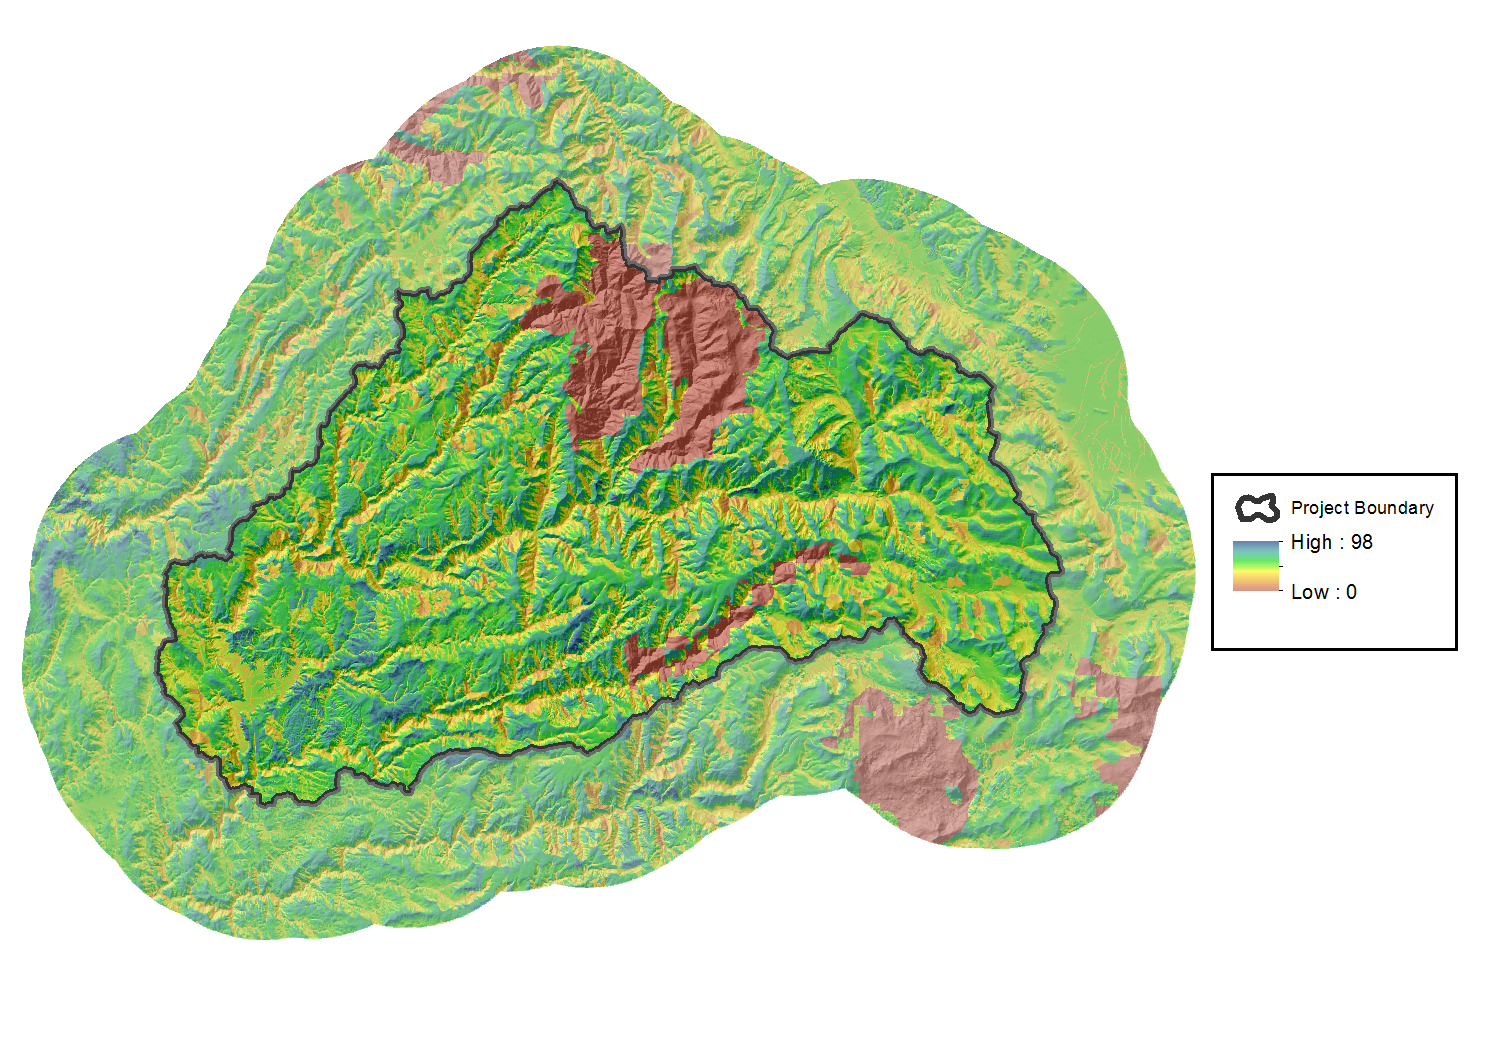
\includegraphics[height=0.4\textheight]{/Users/mmallek/Tahoe/Report2/images/treatpri_rxfire.png}
\caption{Treatment Priority grid for Prescribed Fire treatment class.} 
\label{treatpri_rxfire}
\end{figure}

\begin{figure}
\centering
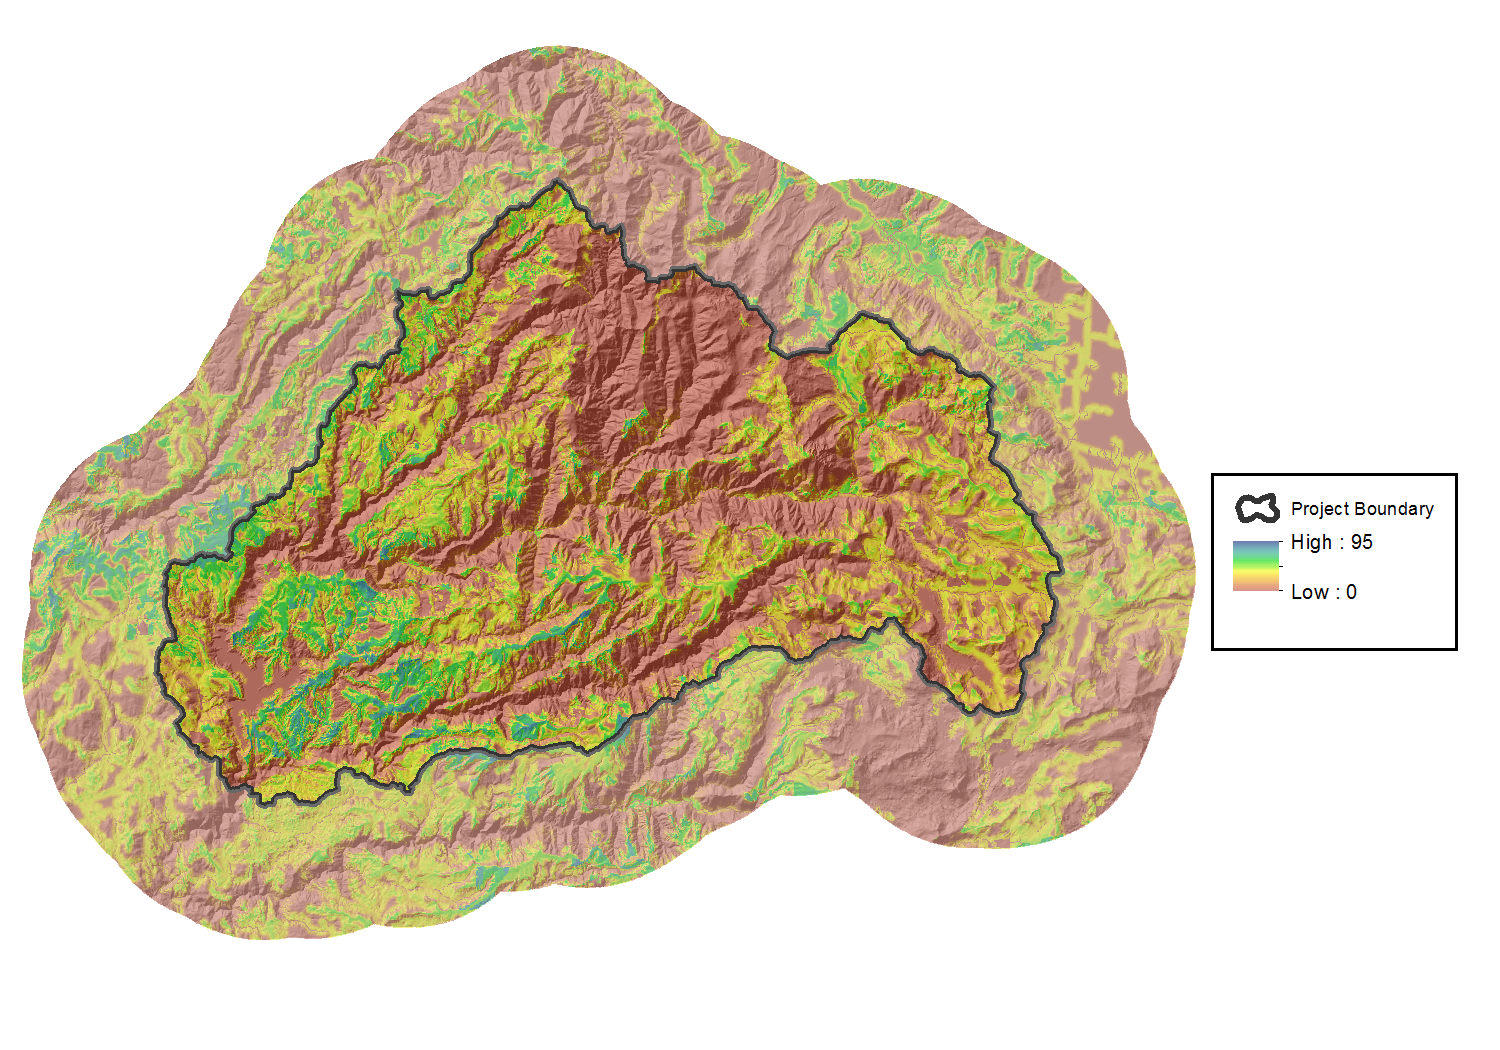
\includegraphics[height=0.4\textheight]{/Users/mmallek/Tahoe/Report2/images/treatpri_undermech.png}
\caption{Treatment Priority grid for Understory Mechanical treatment class.} 
\label{treatpri_undermech}
\end{figure}

\begin{figure}
\centering
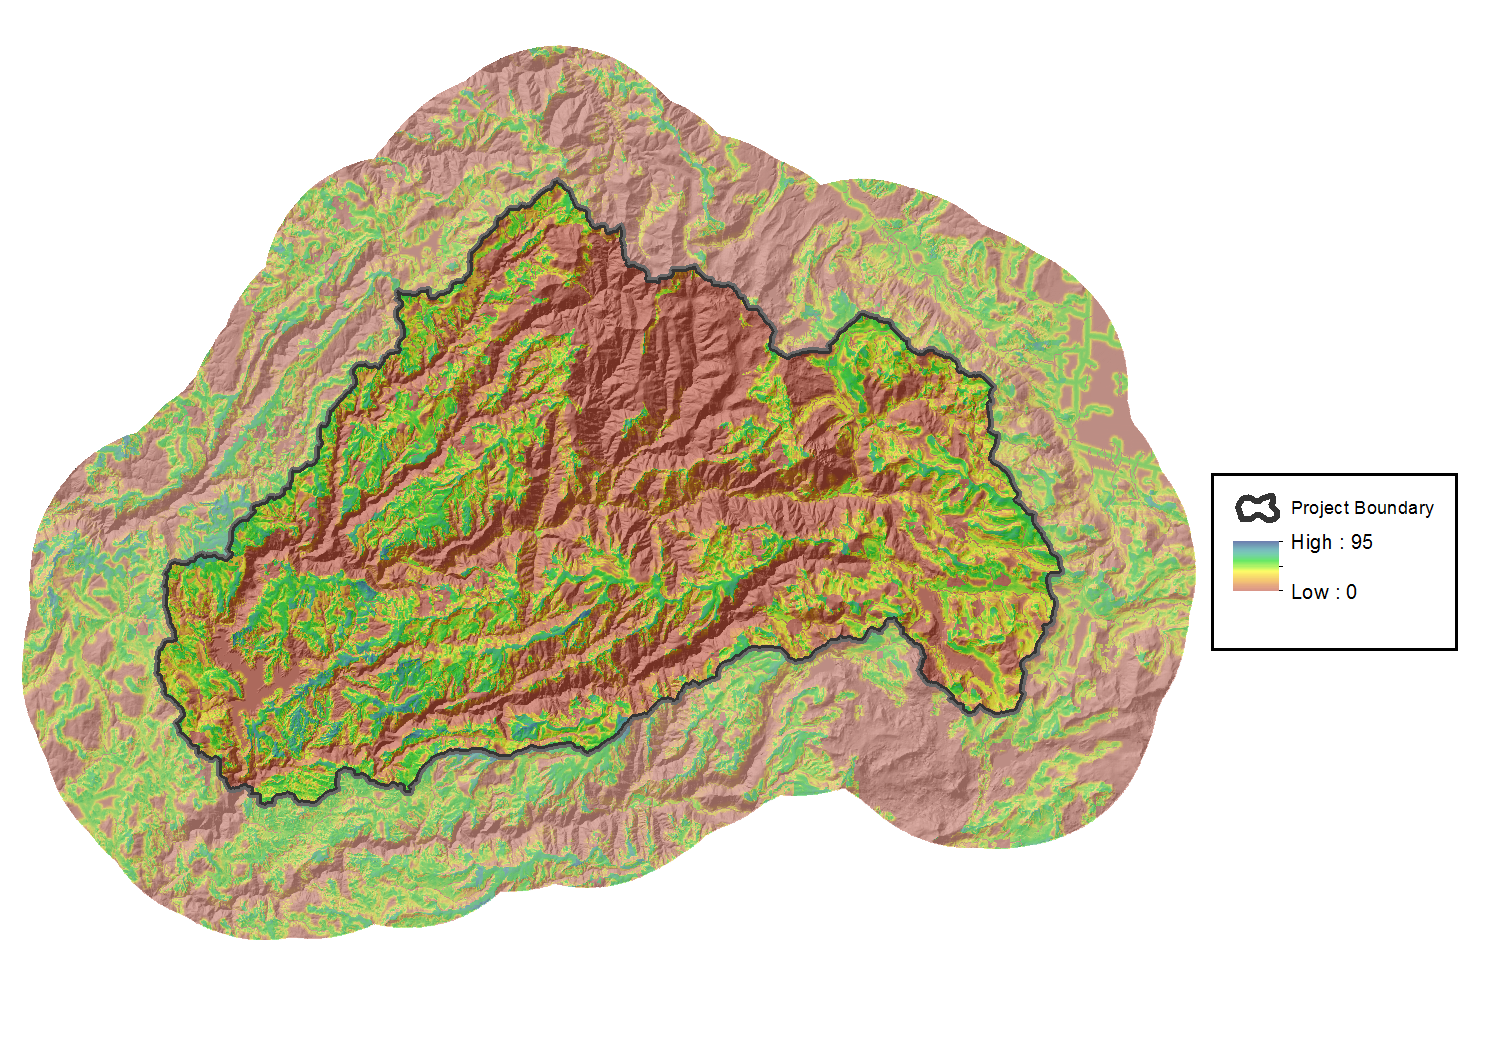
\includegraphics[height=0.4\textheight]{/Users/mmallek/Tahoe/Report2/images/treatpri_thin.png}
\caption{Treatment Priority grid for Thinning treatment class.} 
\label{treatpri_thin}
\end{figure}

\begin{figure}
\centering
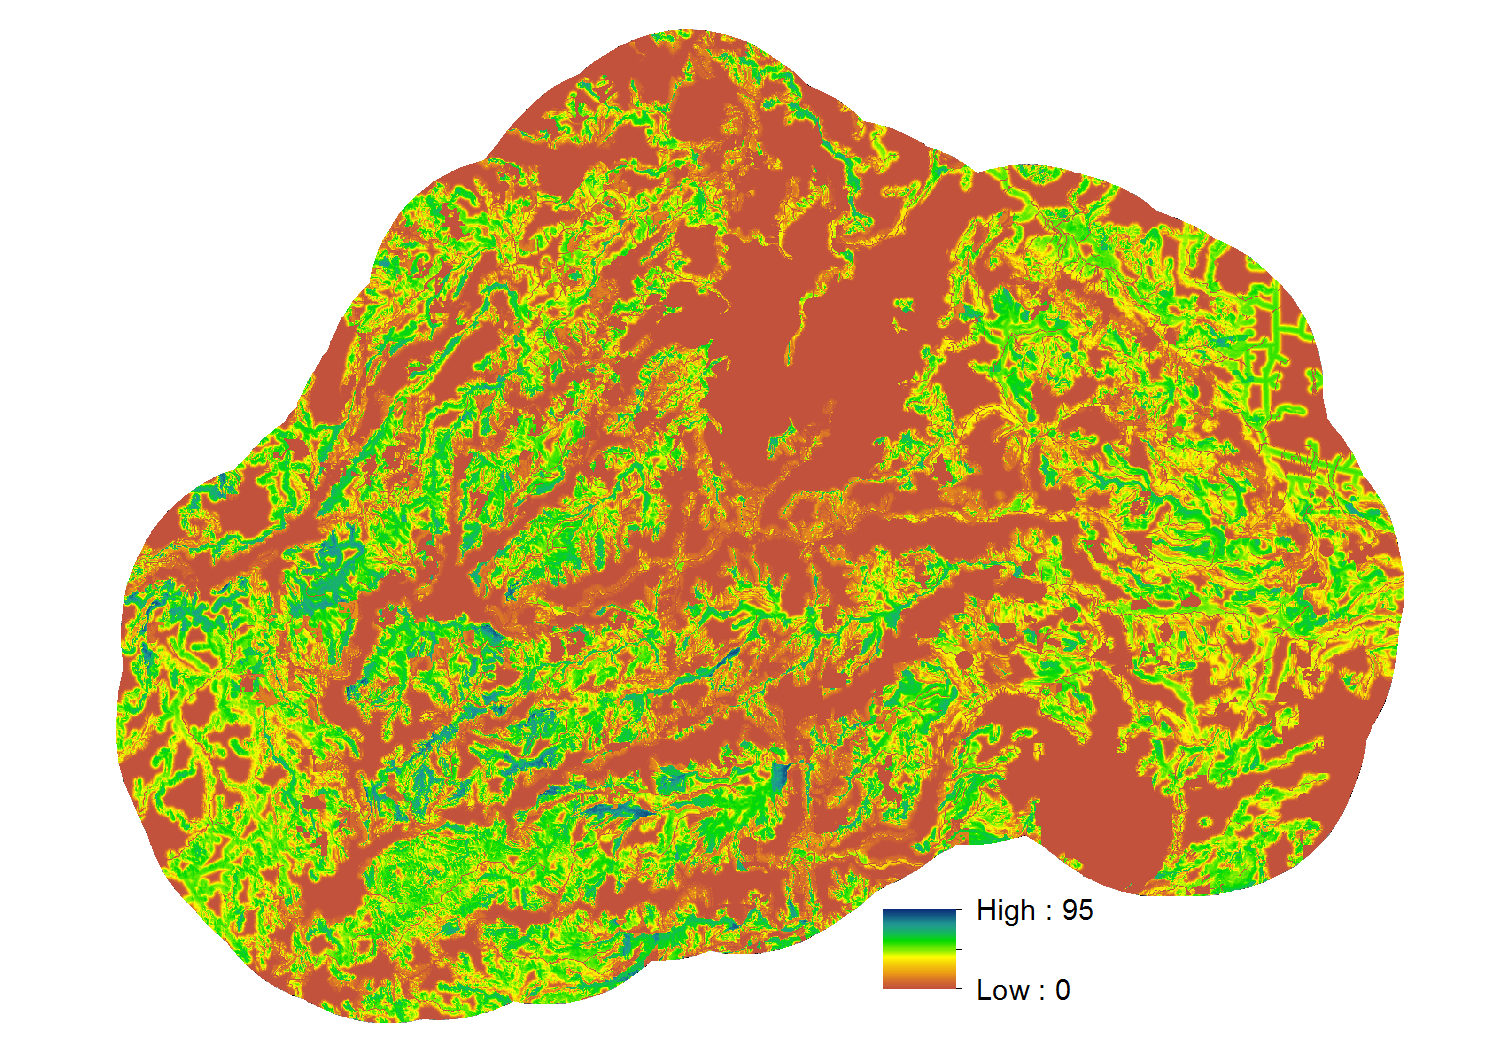
\includegraphics[height=0.4\textheight]{/Users/mmallek/Tahoe/Report2/images/treatpri_matgroup.png}
\caption{Treatment Priority grid for Matrix Thin \& Group Cut treatment class.} 
\label{treatpri_matgroup}
\end{figure}

\subsection{Model Parameterization}

\subsection{Model Calibration}

\subsection{Model Execution}

\subsection{Data Analysis}



 
%\include{3_Geoprocessing} 
%\include{4_RMLandsParameterDevelopment} 
%\include{5_ModelCalibration} 

\backmatter 
\include{glossary} 
\include{notat} 
\bibliographystyle{amsalpha} %The style you want to use for references. 
\bibliography{mr,refs} %The files containing all the articles and books you ever referenced. 
%\printindex %Make an index AUTOMATICALLY 

\end{document} 